The proposed architecture is Half rate DFE because halving the clock frequency results in massive power savings in the clock distribution network and more clean clock with low jitter.

Four comparators because 3 comparators used to distinguish between 4 levels of the PAM-4 signal and one for the error signal for adaptation loop.

\begin{figure}[htbp]
    \centering
    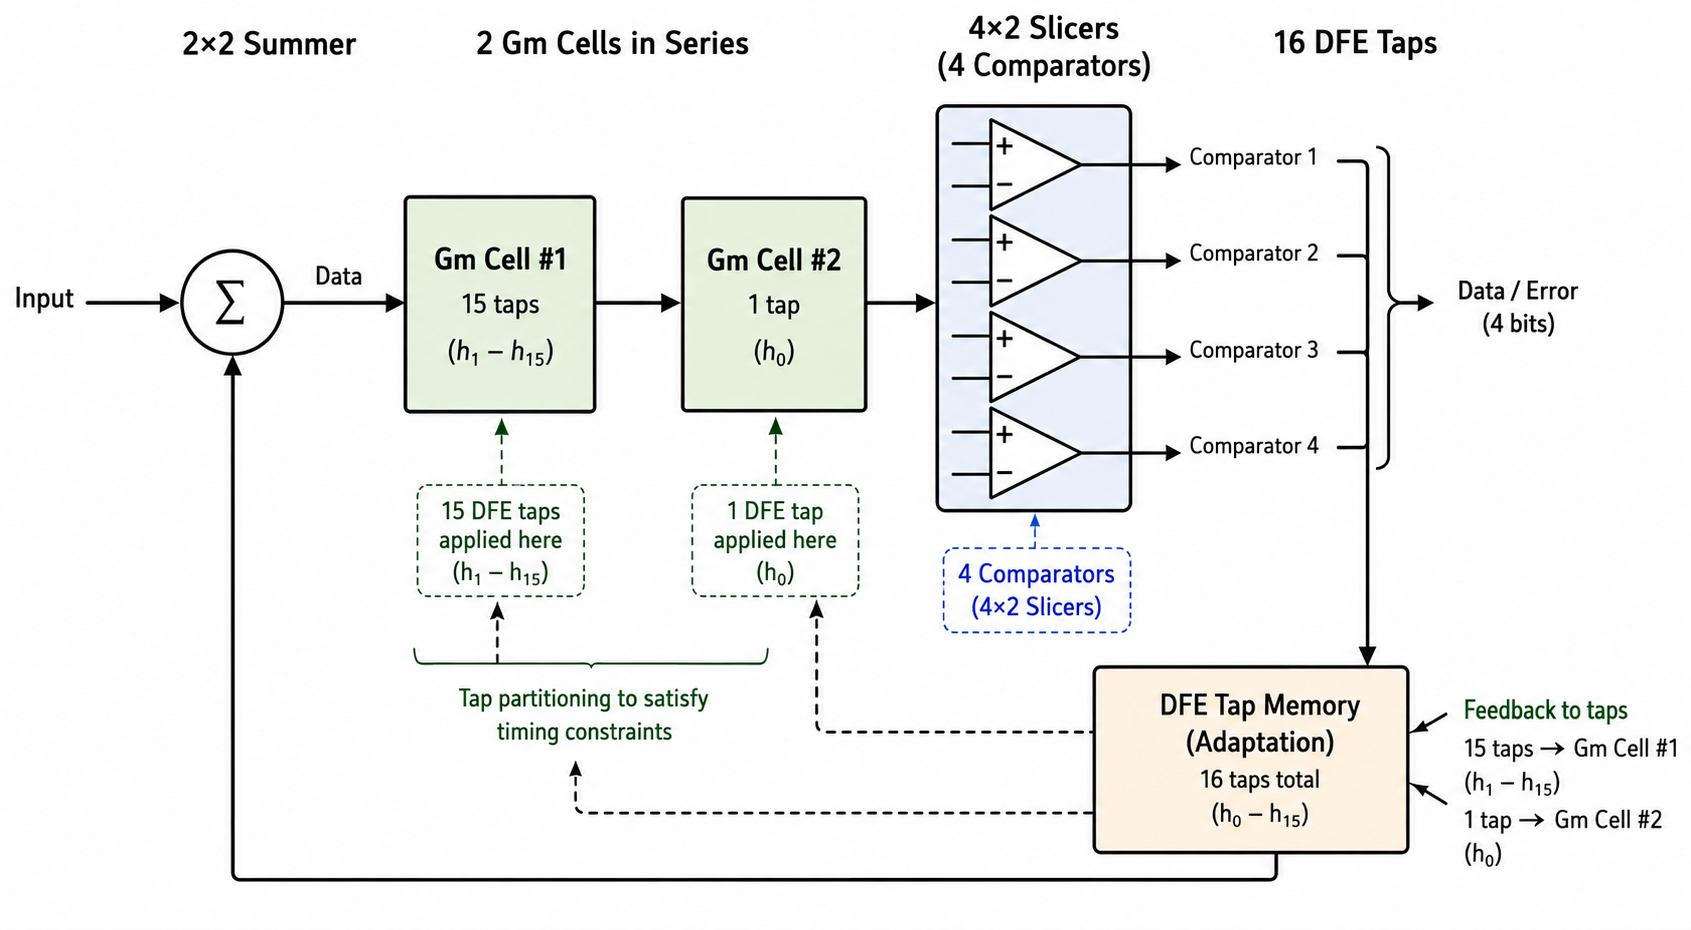
\includegraphics[width=1\textwidth]{img/DFE_img/DFE block.png}
    \caption{Top-level block diagram of the proposed half-rate PAM-4 DFE architecture.}
    \label{fig:image1}
\end{figure}

Standard wants 16 taps, but I don't have the channel response to do so and not the taps value. So, I will try to get close to that.

Thermometer to binary is put after the third latch to avoid critical timing nodes.

\begin{figure}[htbp]
    \centering
    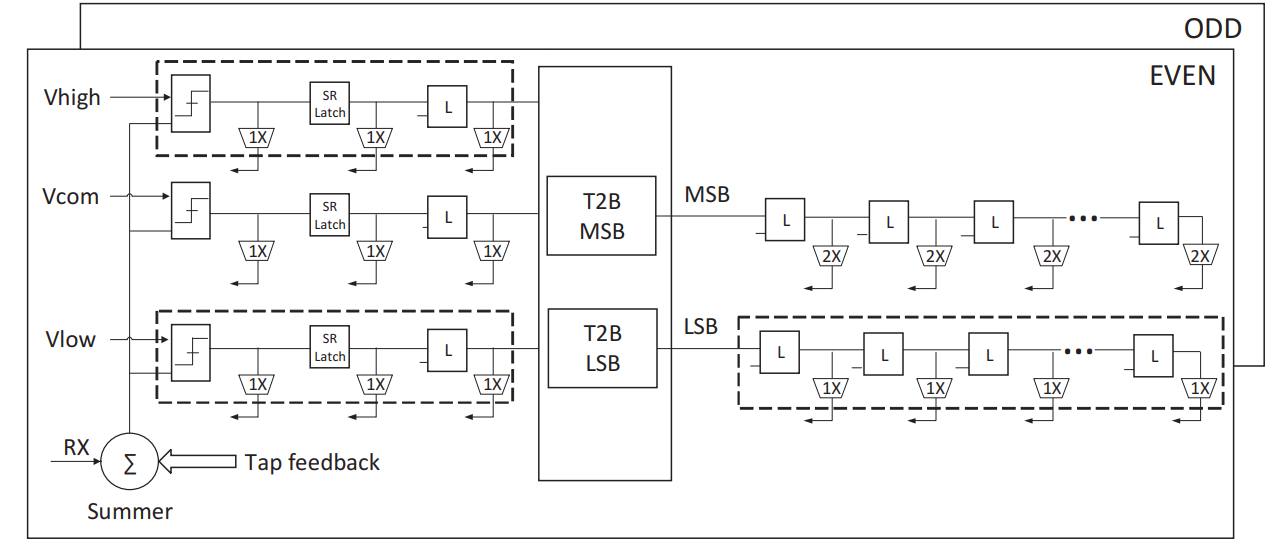
\includegraphics[width=1\textwidth]{img/DFE_img/block.png}
    \caption{16-tap DFE with LSB and MSB paths}
    \label{fig:image2}
\end{figure}
\section{Design of Main Blocks}
\subsection{Comparator}

Azita Latch is the proposed comparator which is CMOS tracking and regeneration to help in high speed and consumes less power than CML.

\begin{figure}[H]
    \centering
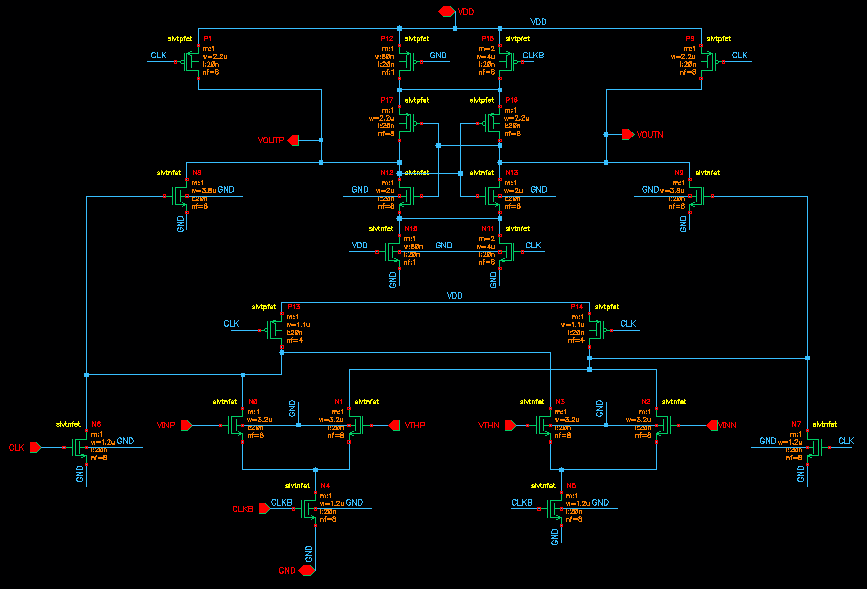
\includegraphics[width=0.9\textwidth]{img/DFE_img/Azita Latch.PNG}
    \caption{Schematic of the Azita Latch (CMOS Track and Regenerate Slicer).}
    \label{fig:azita_latch}
\end{figure}

\subsubsection{Input Common Mode Voltage}

The input common mode voltage is a critical parameter when optimizing the latch for a minimum $T_{cq}$. An increase in the input common mode accelerates the charging and discharging of the internal common-mode nodes. This effectively reduces the duration of the amplification phase, leading to a faster $T_{cq}$. However, beyond a certain threshold, the gain during the amplification phase degrades significantly, which ultimately worsens the $T_{cq}$.

\begin{figure}[H]
    \centering
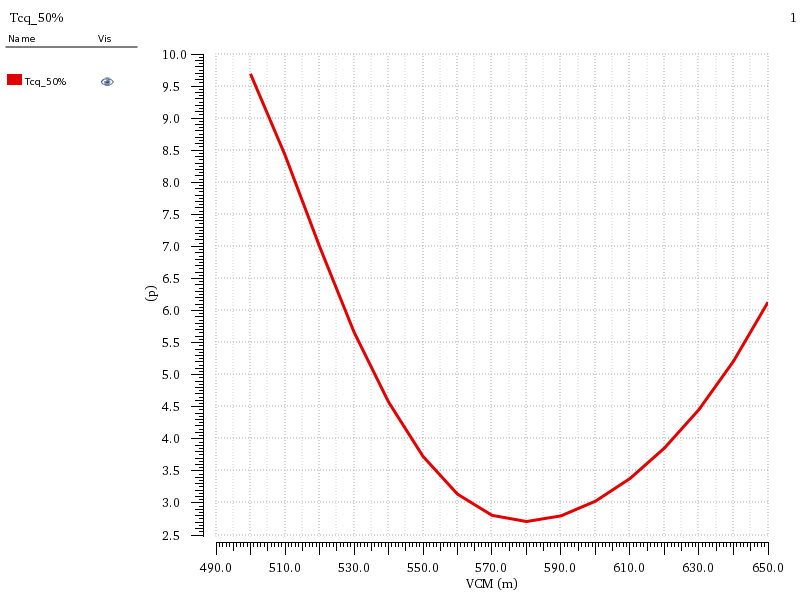
\includegraphics[width=0.7\textwidth]{img/DFE_img/Tcq Vs Vicm.png}
    \caption{Simulation results for $T_{cq}$ versus input common mode voltage.}
    \label{fig:tcq_vcm_graph}
\end{figure}

The simulation results indicate that power consumption is inversely proportional to the input common mode voltage. During the tracking phase, a higher common mode increases the current in the first stage. This higher current is advantageous because it rapidly pulls the intermediate node to a lower voltage, further away from VDD. Consequently, the NMOS input of the second stage is weakened, causing it to conduct less current. Because the path from the VDD to the ground through the NMOS and PMOS at the output dictates the largest contribution to the overall current, this starvation of the second stage significantly reduces the total power consumption.
\begin{figure}[H]
    \centering
    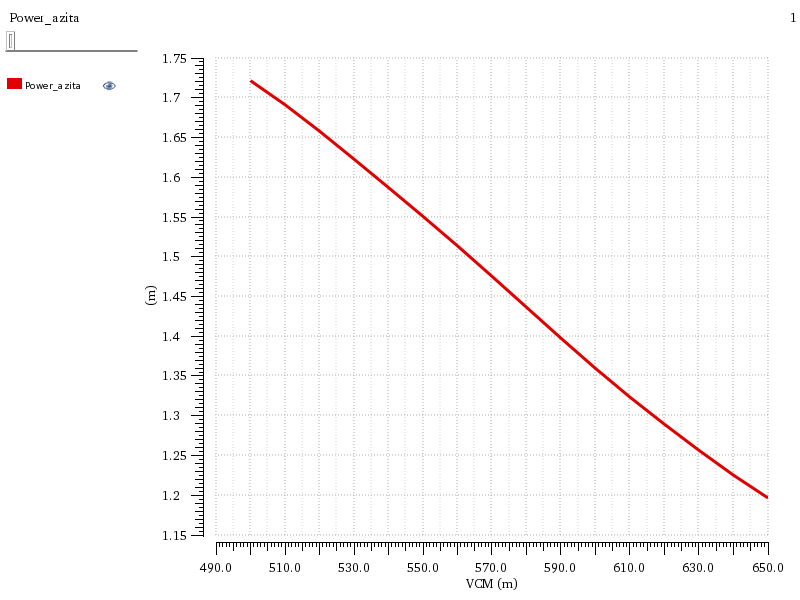
\includegraphics[width=0.7\textwidth]{img/DFE_img/Power Vs VICM.png}
    \caption{Power Vs VICM}
    \label{fig:Power Vs VICM}
\end{figure}

\subsubsection{Setup Time ($T_{setup}$)}

The setup time ($T_{setup}$) of the comparator is characterized using two distinct methodologies:

The first approach involves sweeping the delay between the input data signal and the clock edge to identify the point at which $T_{dc} + T_{cq}$  ($T_{dq}$) is minimum. 
This is the point at which the slope of $T_{cq}$ Vs $T_{dc}$ = -1 that indicates an increase/decrease $T_{dc}$ is counteracted by a decrease/increase $T_{cq}$ with the same magnitude that makes this point minimum. After or before that point, the change is not the same value.

At this point, we consider $T_{dc}$ equal to $T_{setup}$. 
$T_{setup}$ = 11.25 ps.
\begin{figure}[H]
    \centering
  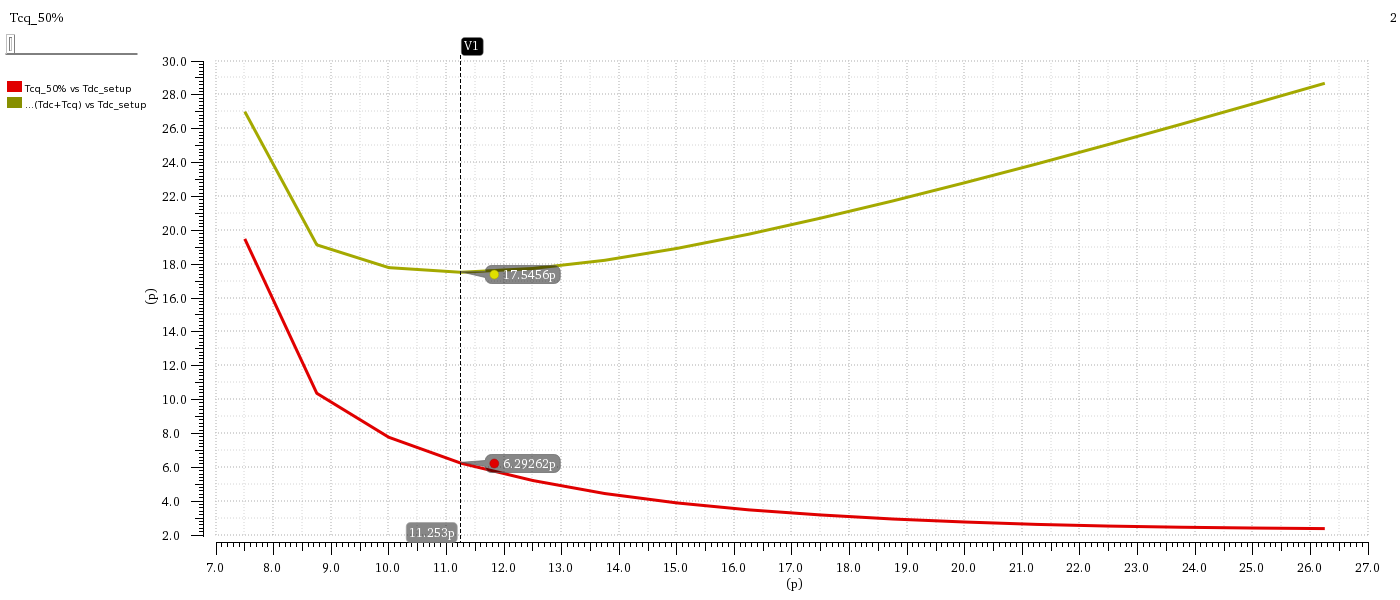
\includegraphics[width=0.7\textwidth]{img/DFE_img/Tsetup.png}
    \caption{Plot of $T_{cq}$ and $T_{dc}+T_{cq}$ versus the delay between input signal and CLK.}
    \label{fig:tsetup_graph}
\end{figure}

The second methodology extracts the sampling aperture from the Impulse Sensitivity Function (ISF), utilizing the definition that $T_{setup}$ is approximately equal to 90\% of the sampling aperture. The measurement setup, based on the methodology presented in [Jeeradit VLSI'08], relies on finding the specific offset voltage that forces the comparator into metastability for a given input-to-clock delay.

\begin{figure}[H]
    \centering
    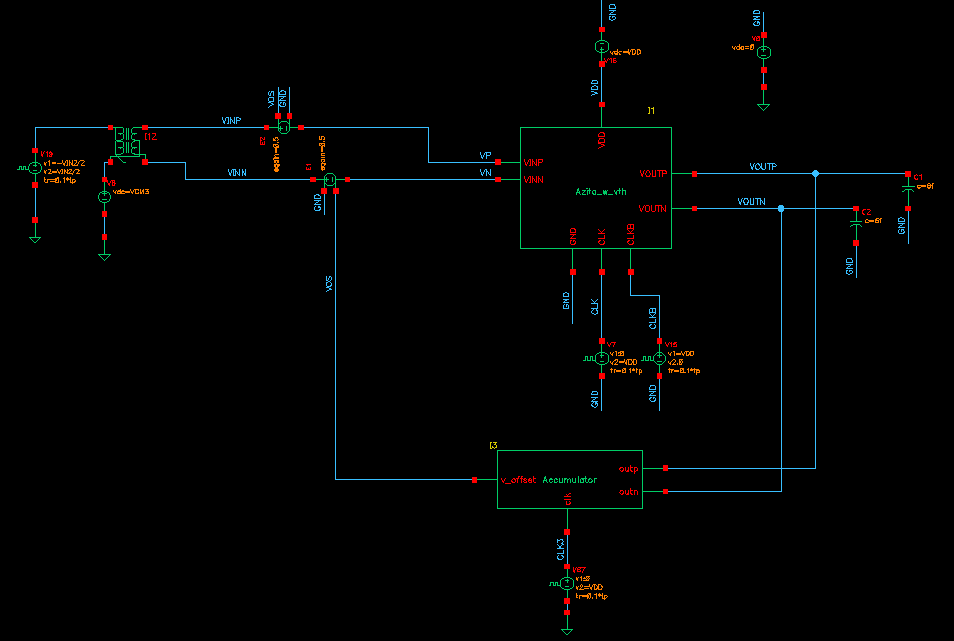
\includegraphics[width=0.8\textwidth]{img/DFE_img/ISF TB.png}
    \caption{Schematic of the measurement setup used for ISF extraction.}
    \label{fig:setup_schematic}
\end{figure}

To automate this, an accumulator implemented in Verilog-A acts as an integrator, continuously increasing the applied offset voltage until the comparator enters metastability and its output alternates. This search process is repeated across a sweep of delay values.

The resulting curve of offset voltage versus delay is then imported into MATLAB. The data is processed to normalize the Step Sensitivity Function (SSF). Finally, the data is interpolated and smoothed using a digital filter to produce a clean ISF curve upon taking the derivative of the SSF.

\begin{figure}[H]
    \centering
    \begin{minipage}{0.45\linewidth}
        \centering
        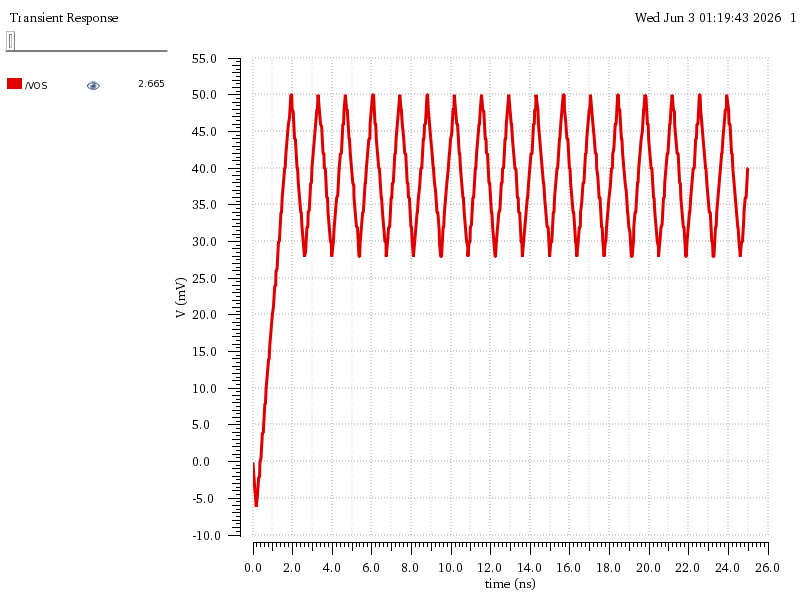
\includegraphics[width=\linewidth]{img/DFE_img/VOS_ISF.png}
        \caption{VOS at certain delay value}
        \label{fig:slide17_1}
    \end{minipage}\hfill%
    \begin{minipage}{0.45\linewidth}
        \centering
        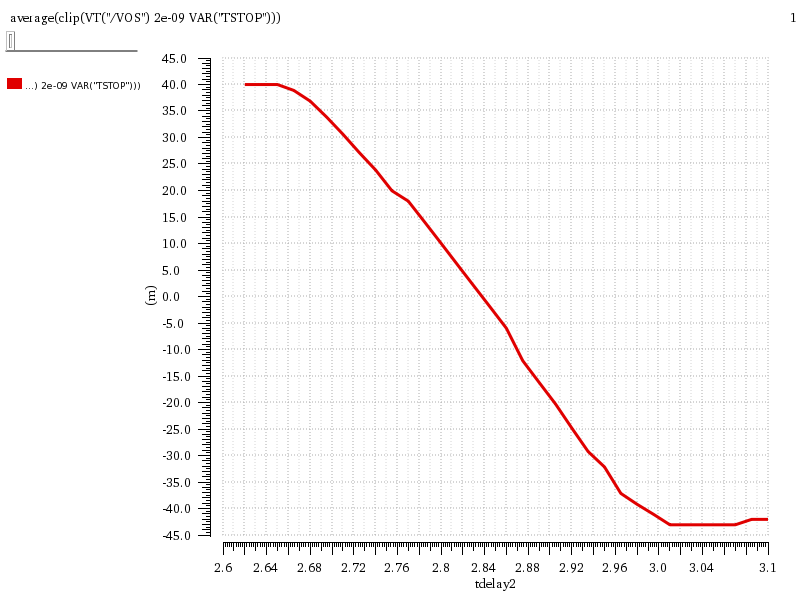
\includegraphics[width=\linewidth]{img/DFE_img/VOS_across_delay.png}
        \caption{VOS across delay}
        \label{fig:slide17_2}
    \end{minipage}
\end{figure}

\begin{figure}[H]
    \centering
    \begin{minipage}{0.48\textwidth}
        \centering
        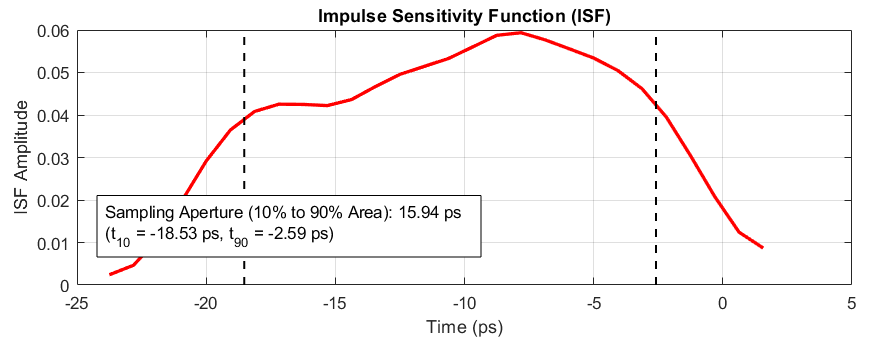
\includegraphics[width=\linewidth]{img/DFE_img/Gaussian_window_7.PNG}
        \caption{Gaussian with window size = 7}
        \label{fig:slide18_1}
    \end{minipage}\hfill%
    \begin{minipage}{0.48\textwidth}
        \centering
        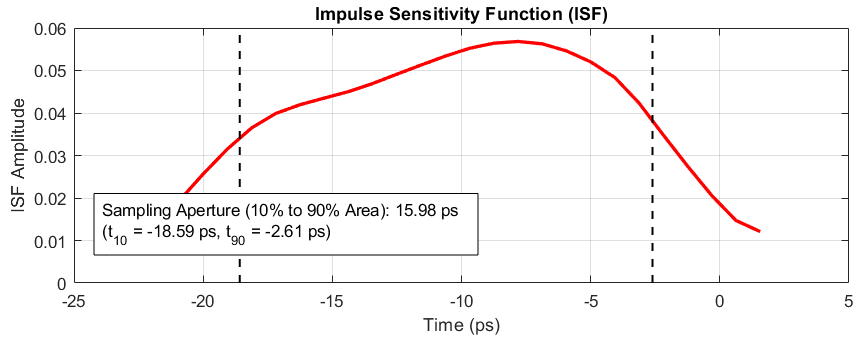
\includegraphics[width=\linewidth]{img/DFE_img/Gaussian_window_12.PNG}
        \caption{Gaussian with window size = 12}
        \label{fig:slide18_2}
    \end{minipage}

    \vspace{0.5cm} % Adds a neat gap between the top and bottom rows

    \begin{minipage}{0.48\textwidth}
        \centering
        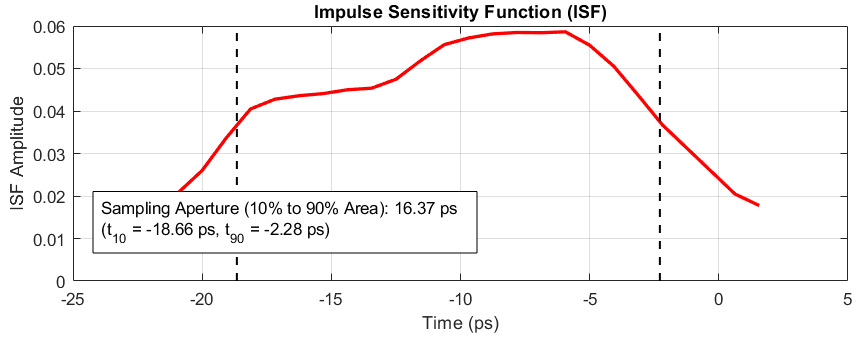
\includegraphics[width=\linewidth]{img/DFE_img/sgolay_window_11.PNG}
        \caption{Savitzky-Golay Filter with window size = 11 }
        \label{fig:slide18_3}
    \end{minipage}\hfill%
    \begin{minipage}{0.48\textwidth}
        \centering
        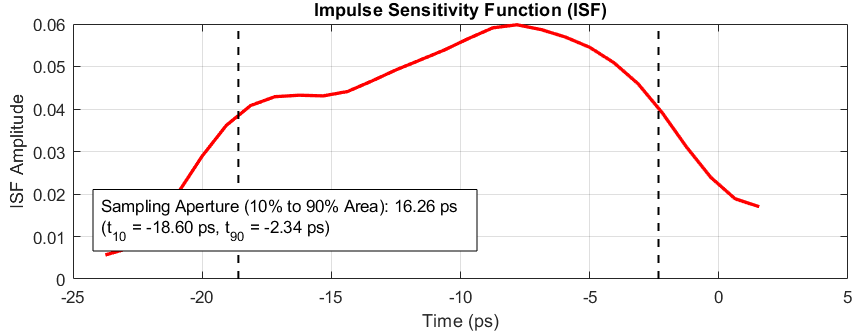
\includegraphics[width=\linewidth]{img/DFE_img/smoothing spline.PNG}
        \caption{Smoothing Spline with SmoothingParam = 0.3 }
        \label{fig:slide18_4}
    \end{minipage}
\end{figure}

$T_{setup}$ according to this method = 0.9 * 16 ps = 14.4 ps

\subsubsection{Hold Time ($T_{hold}$)}

The hold time ($T_{hold}$) is calculated using the same methodology applied to $T_{setup}$, which involves sweeping the delay between the input data signal and the clock edge. However, for this characterization, the measurement is taken while the input signal is falling and the output $Q$ is rising (in contrast to the $T_{setup}$ measurement, where both the input and $Q$ were rising). 

Based on this methodology, the hold time is evaluated to be:
\begin{equation}
    T_{hold} = -T_{dc} = -4 \text{ ps}
\end{equation}

\begin{figure}[H]
    \centering
    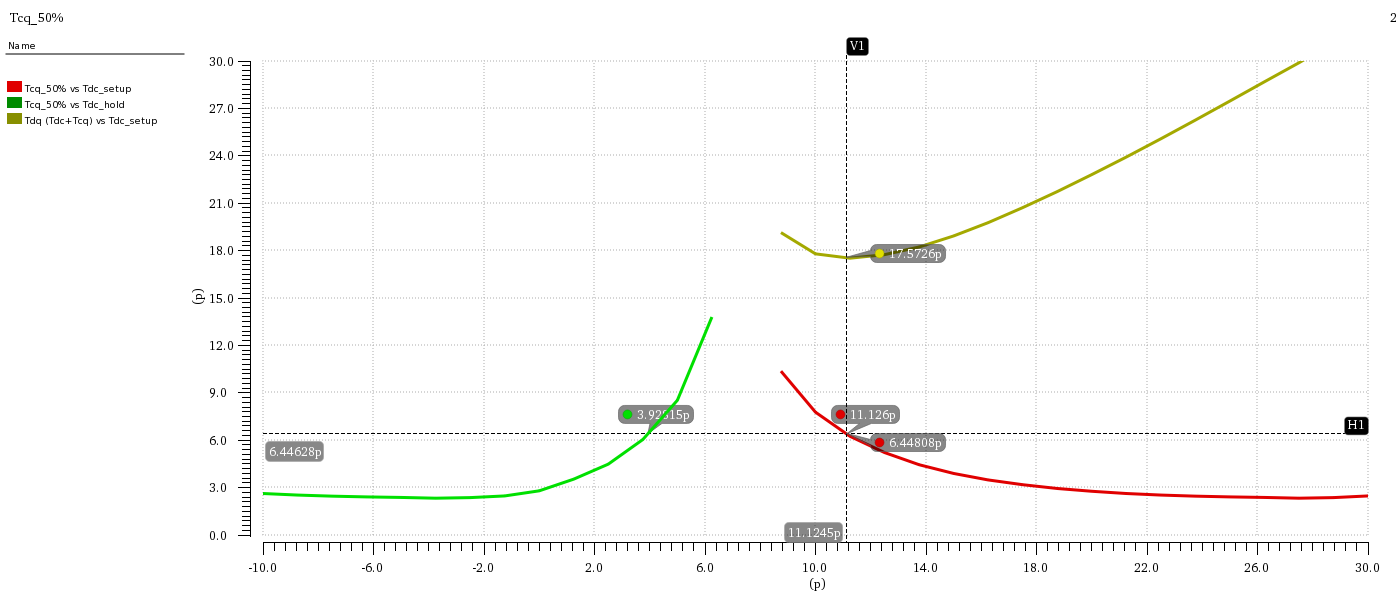
\includegraphics[width=0.9\textwidth]{img/DFE_img/Thold.png}
    \caption{Hold time measurement showing $T_{hold}$ evaluated at -4 ps.}
    \label{fig:thold_measurement}
\end{figure}

\subsubsection{Input Referred Noise}

The input referred noise of the comparator is measured using two distinct methodologies:

\textbf{1. Using CDF Curve Analysis:}

The first methodology utilizes a Cumulative Distribution Function (CDF) curve. The input voltage ($V_{in}$) is swept from -4 mV to 4 mV with a step size of 0.3 mV. A transient noise analysis is then applied with a stop time ($T_{stop}$) of 40 ns. The probability of outputting a logic '1' at each step is calculated using a custom Verilog-A code block. These probability results are subsequently imported into MATLAB, where they are fitted to a Gaussian CDF curve to extract the standard deviation ($\sigma$), representing the noise. From this measurement, the input referred noise is found to be 1.314 mV.

\begin{figure}[H]
    \centering
    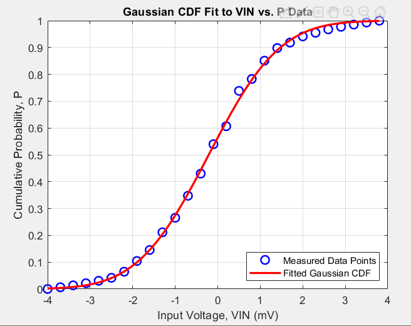
\includegraphics[width=0.4\textwidth]{img/DFE_img/input referred noise.png}
    \caption{Gaussian CDF curve fitting for input referred noise measurement.}
    \label{fig:noise_cdf}
\end{figure}

\textbf{2. Using PSS and Pnoise Analysis:}

The second methodology employs Periodic Steady-State (PSS) and Periodic Noise (Pnoise) analyses. As detailed in the methodologies by [J. Kim TCAS-I'09] and [Azita Emami JSSC'20], the input referred noise can be derived directly from the Signal-to-Noise Ratio (SNR). This technique requires selecting a specific time of observation at which the large-signal nonlinearity of the comparator has not yet led to the compression of the output noise power.

The configurations used for the PSS and Pnoise simulations are shown below:
\begin{figure}[H]
    \centering
    % Top Row: PSS Setup centered alone
    \begin{minipage}{0.55\textwidth}
        \centering
        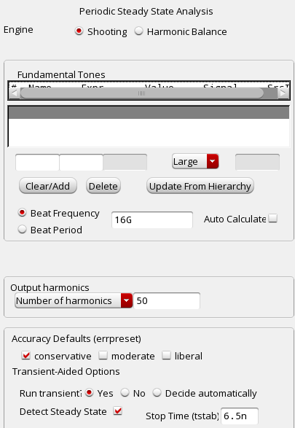
\includegraphics[width=0.6\linewidth]{img/DFE_img/PSS_SETUP.png}
        \caption{First PSS setup configuration.}
        \label{fig:pss_setup_1}
    \end{minipage}

    \vspace{0.1cm} % This controls the vertical gap between the top and bottom rows

    % Bottom Row: Two Pnoise setups side-by-side
    \begin{minipage}{0.48\textwidth}
        \centering
        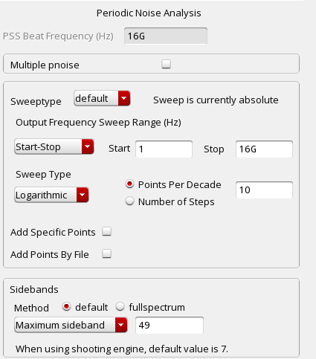
\includegraphics[width=0.7\linewidth]{img/DFE_img/Pnoise_setup.png}
        \caption{Pnoise setup configuration.}
        \label{fig:pss_setup_2}
    \end{minipage}\hfill%
    \begin{minipage}{0.48\textwidth}
        \centering
        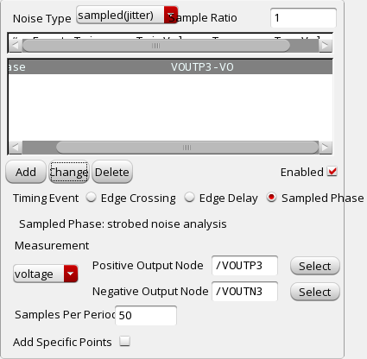
\includegraphics[width=0.6\linewidth]{img/DFE_img/Pnoise_SETUP_2.png}
        \caption{Second Pnoise setup configuration.}
        \label{fig:pss_setup_3}
    \end{minipage}
\end{figure}

The output integrated noise and the corresponding SNR are then extracted to calculate the final input referred noise:

\begin{figure}[H]
    \centering
    \begin{minipage}{0.48\textwidth}
        \centering
        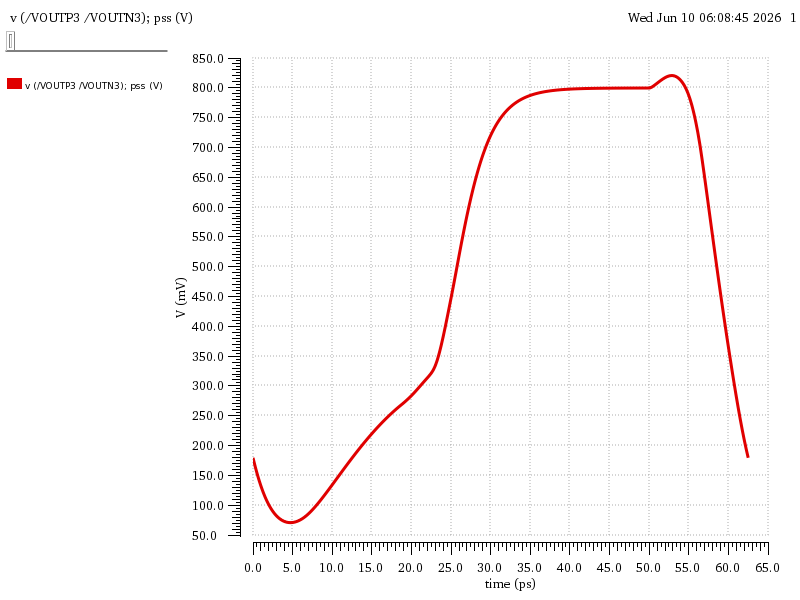
\includegraphics[width=0.9\linewidth]{img/DFE_img/OUTPUT COMPARATOR PSS.png}
        \caption{ Output diff voltage of comparator from PSS.}
        \label{fig:slide22_noise}
    \end{minipage}\hfill%
    \begin{minipage}{0.48\textwidth}
        \centering
        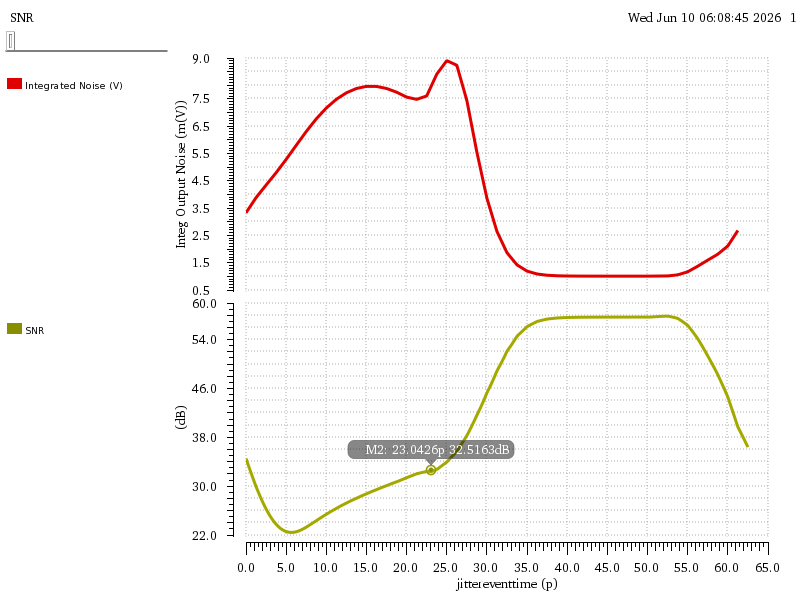
\includegraphics[width=0.9\linewidth]{img/DFE_img/SNR and Noise.png}
        \caption{Output integrated noise and SNR from Pnoise }
        \label{fig:slide22_snr}
    \end{minipage}
\end{figure}

Based on these simulation results, for an SNR of 32.516 dB and a differential input voltage of 50 mV, the calculated input referred noise is 1.18 $V_{rms}$.

\subsubsection{Input Referred Offset}

The input referred offset of the comparator is evaluated using two methodologies:

\textbf{1. CDF Curve Analysis:}

Similarly to the input referred noise measurement, the first method utilizes a Cumulative Distribution Function (CDF) curve. The input voltage ($V_{in}$) is swept from -25 mV to 25 mV with a step size of 10 mV, and the transient stop time ($T_{stop}$) is set to 20 ps. The resulting CDF curve is plotted and subsequently imported into MATLAB. The data is then fitted to a Gaussian distribution to extract the standard deviation ($\sigma$), representing the offset. Based on this methodology, the input referred offset is determined to be 15.213 mV.

\begin{figure}[H]
    \centering
    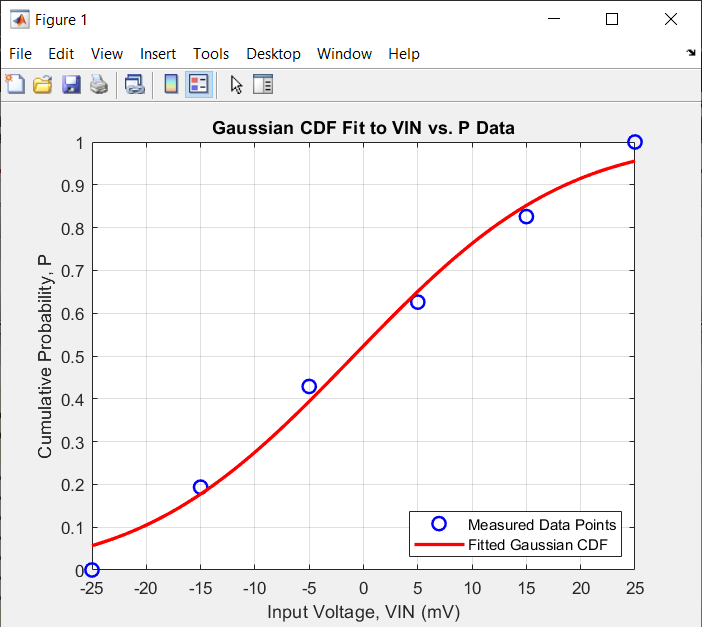
\includegraphics[width=0.5\textwidth]{img/DFE_img/Offset_graph.PNG}
    \caption{Gaussian CDF curve fitting for input referred offset measurement.}
    \label{fig:offset_cdf}
\end{figure}

\textbf{2. Using an Accumulator with Monte Carlo Analysis:}

The second methodology employs an accumulator-based feedback loop in conjunction with Monte Carlo simulations. For each Monte Carlo iteration, the feedback loop acts as an integrator, continuously adjusting the applied offset voltage ($V_{OS}$) until the comparator is forced into a metastable state. The voltage recorded at the exact onset of metastability represents the specific input referred offset for that individual simulation run.


\begin{figure}[H]
    \centering
    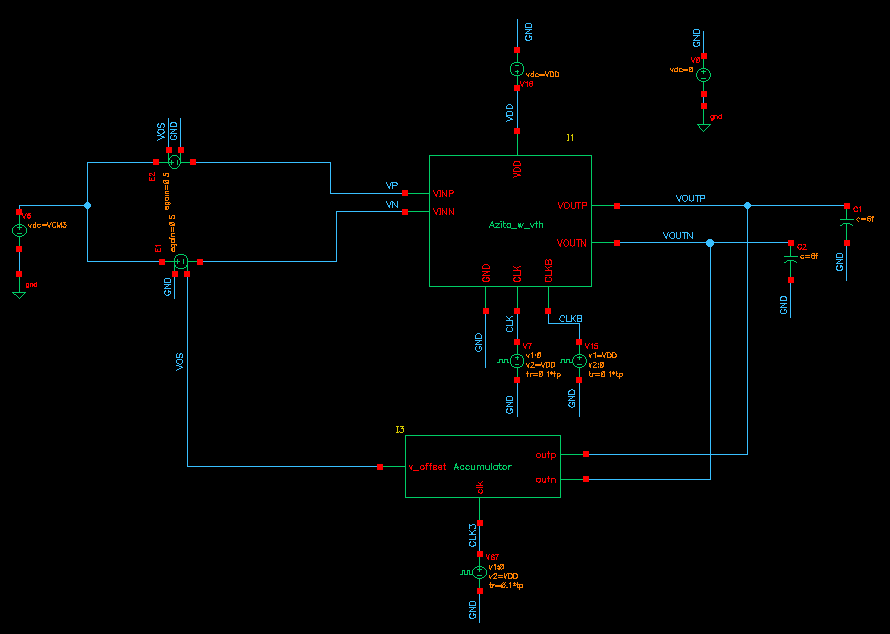
\includegraphics[width=0.7\textwidth]{img/DFE_img/Input referred offset TB.png}
    \caption{Histogram of the input referred offset obtained from Monte Carlo simulations.}
    \label{fig:offset_histogram}
\end{figure}

By repeating this tracking process across all Monte Carlo iterations, a comprehensive distribution of the extracted offset voltages is collected. A histogram of these data points is then plotted to evaluate the statistical variance across the iterations. 
Based on this distribution, the overall input referred offset is calculated to be 14.97 mV.

\begin{figure}[H]
    \centering
    \begin{minipage}{0.45\textwidth}
        \centering
        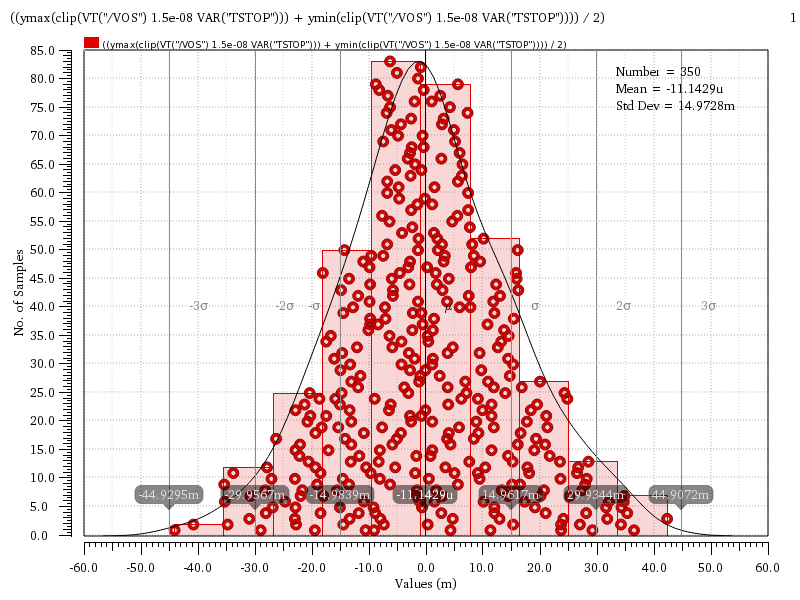
\includegraphics[width=1.2\linewidth]{img/DFE_img/input referred offset.png}
        \caption{Schematic of the accumulator-based testbench.}
        \label{fig:offset_testbench}
    \end{minipage}\hfill%
    \begin{minipage}{0.45\textwidth}
        \centering
        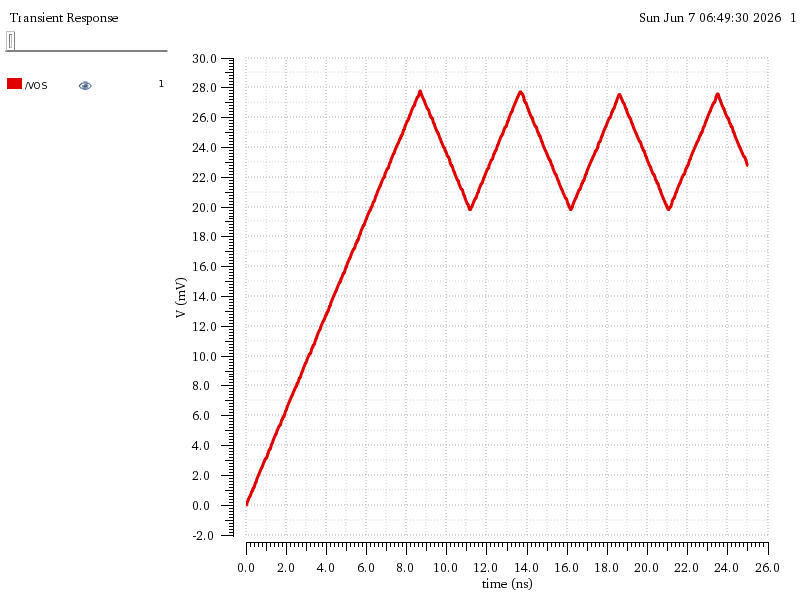
\includegraphics[width=1.2\linewidth]{img/DFE_img/VOS_OFFSET.png}
        \caption{Transient waveform showing $V_{OS}$ converging during a single run.}
        \label{fig:vos_single_run}
    \end{minipage}
\end{figure}
\subsubsection{$T_{cq}$ Across Corners}

The clock-to-Q delay ($T_{cq}$) is measured across 13 distinct simulation corners. It is important to note that these conditions account for supply voltage variations ranging from -7\% to +5\% of the nominal 0.8 V supply.

\begin{figure}[H]
    \centering
    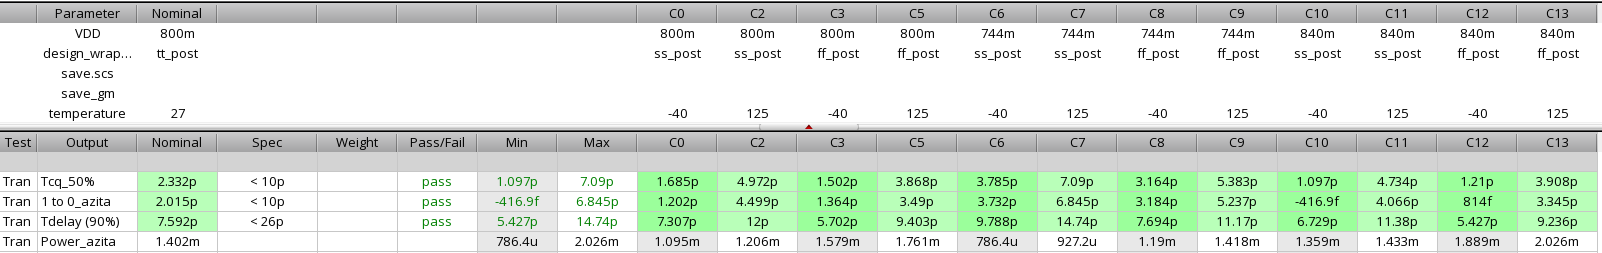
\includegraphics[width=\textwidth]{img/DFE_img/Tcq across corners.PNG}
    \caption{Simulation results demonstrating $T_{cq}$ variations across 13 operating corners.}
    \label{fig:tcq_corners}
\end{figure}

\subsection{C2MOS}

The schematic of the Clocked CMOS (C2MOS) latch is presented below.

\begin{figure}[H]
    \centering
    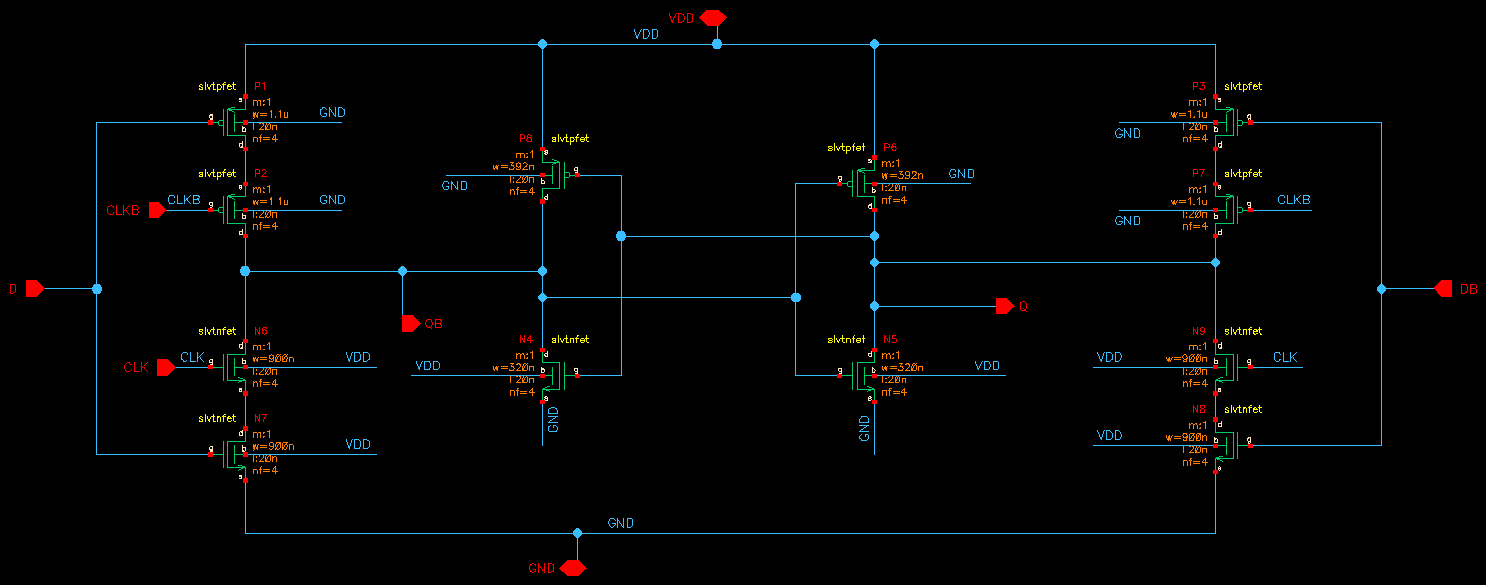
\includegraphics[width=1\textwidth]{img/DFE_img/C2MOS Latch.png}
    \caption{Schematic of the C2MOS latch.}
    \label{fig:c2mos_schematic}
\end{figure}

Similar to the Azita comparator, the C2MOS latch operates using a two-phase clocking scheme consisting of tracking and regeneration phases. This architecture is highly advantageous for achieving an exceptionally low clock-to-Q delay ($T_{cq}$). In certain conditions, the $T_{cq}$ can even reach negative values. A negative $T_{cq}$ indicates that the output successfully reaches 50\% of its final voltage state during the tracking phase, prior to the onset of the regeneration phase.

The simulated clock-to-Q delays for the C2MOS latch transitions are evaluated as follows:
\begin{itemize}
    \item $T_{cq}$ (High-to-Low transition) = -13.87 ps
    \item $T_{cq}$ (Low-to-High transition) = -13.17 ps
\end{itemize}

\begin{figure}[H]
    \centering
    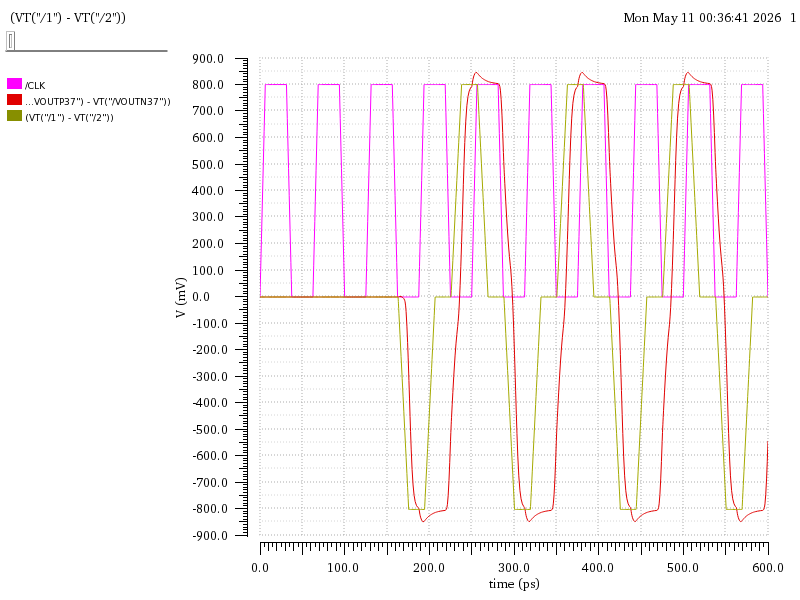
\includegraphics[width=0.8\textwidth]{img/DFE_img/graphs.png}
    \caption{Transient simulation results demonstrating the negative $T_{cq}$ for both High-to-Low and Low-to-High transitions.}
    \label{fig:c2mos_simulation}
\end{figure}

\subsection{C2MOS Latches Cascaded after Azita's Comparator}

The testbench schematic for the C2MOS latches cascaded immediately after the Azita comparator is illustrated below.

\begin{figure}[H]
    \centering
    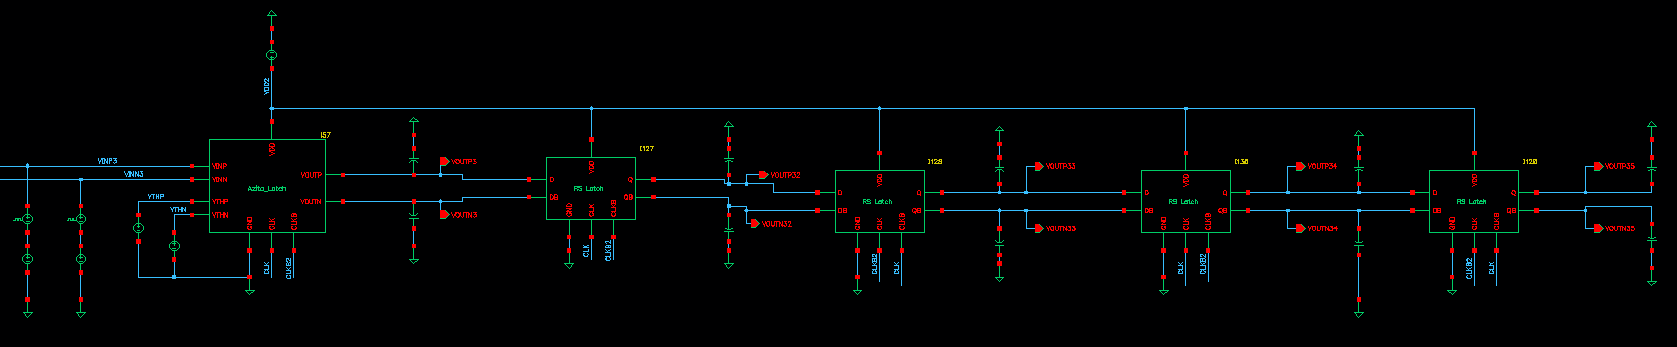
\includegraphics[width=\textwidth]{img/DFE_img/1Azita, all C2MOS (Last).PNG}
    \caption{Testbench schematic of the C2MOS latches cascaded after the Azita comparator.}
    \label{fig:cascaded_c2mos_tb}
\end{figure}

To ensure robust timing performance under varying conditions, the clock-to-Q delay ($T_{cq}$) for this cascaded configuration is measured comprehensively across the simulation corners.

\begin{figure}[H]
    \centering
    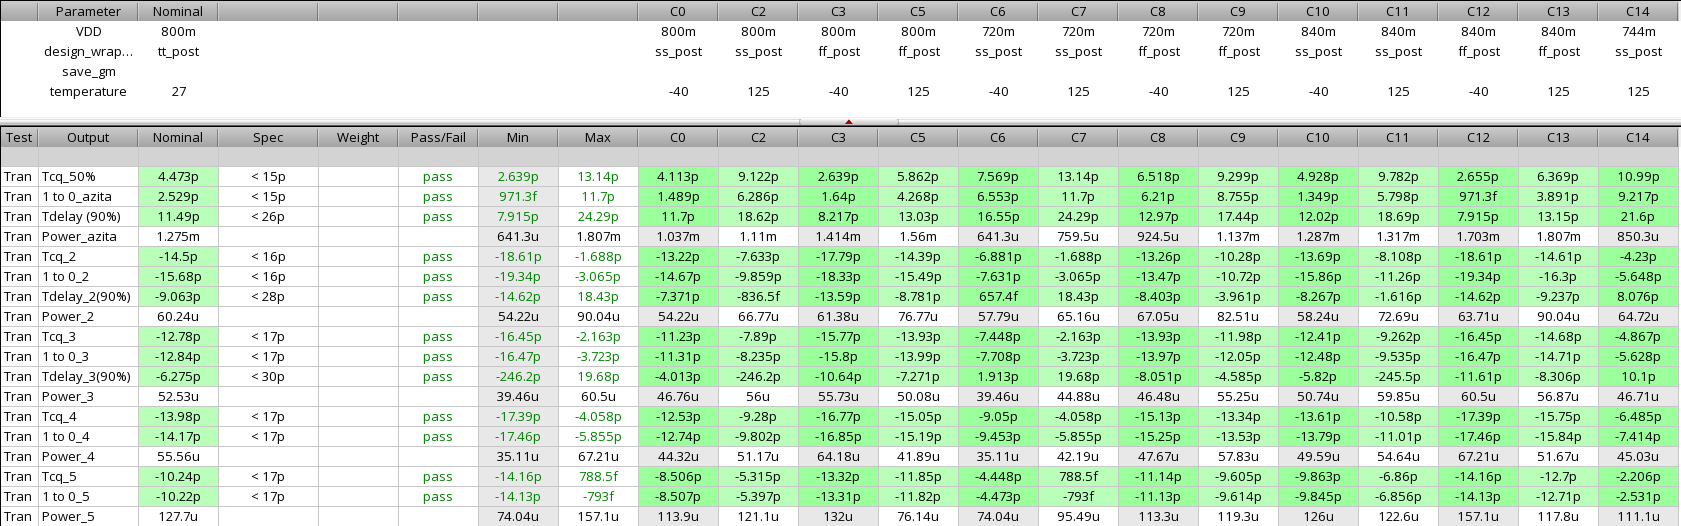
\includegraphics[width=\textwidth]{img/DFE_img/1Azita, all C2MOS_results (Last).PNG}
    \caption{Simulation results demonstrating $T_{cq}$ variations for the cascaded architecture across operating corners.}
    \label{fig:cascaded_tcq_corners}
\end{figure}

\subsection{Differential Pair}

\subsubsection{Hand Analysis}

The design of the differential pair requires careful selection of parameters to meet the specific timing and voltage swing requirements of the system. The hand analysis and structural targets are summarized as follows:

\begin{itemize}
    \item The load resistance ($R_L$) is chosen to be 110 $\Omega$ to achieve a 95\% settling time of less than 12 ps.
    \item The input common mode voltage is set to 0.54 V.
    \item The target output common mode voltage is designed to be 0.6 V.
    \item An output swing greater than 300 mV (differential peak-to-peak) is established to provide sufficient margin between the signal and the threshold voltage ($V_{th}$) of the subsequent comparator, which fundamentally aids in optimizing $T_{cq}$.
    \item The limits of the Common Mode Input Range (CMIR)  are defined as $CMIR_{Low} = 0.56\text{ V} - V_{GS,in}$ and $CMIR_{High} = 0.56\text{ V} + V_{th,in}$.
    \item The maximum supported input range is specified as 400 mV differential peak-to-peak.
    \item The target differential voltage gain is set to be $>0.75$ V/V.
    \item Source degeneration is implemented to effectively linearize the signal, ensuring a robust Ratio of Linear Margin (RLM).
\end{itemize}

\begin{figure}[H]
    \centering
    \begin{minipage}{0.48\textwidth}
        \centering
        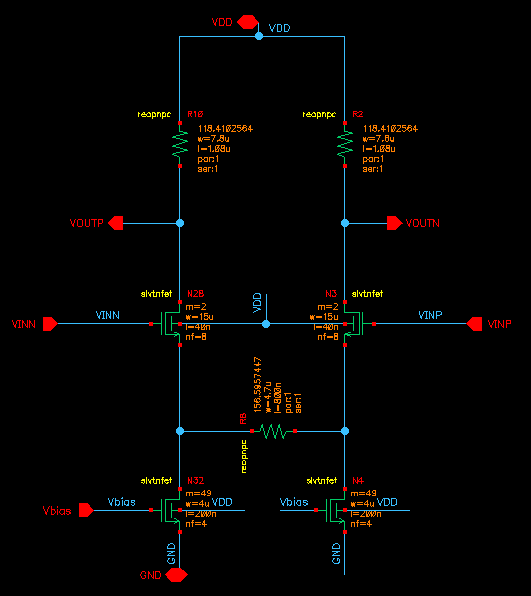
\includegraphics[width=\linewidth]{img/DFE_img/1st GM cell.png}
        \caption{Schematic of the first $G_m$ cell.}
        \label{fig:gm_cell_1_schematic}
    \end{minipage}\hfill%
    \begin{minipage}{0.48\textwidth}
        \centering
        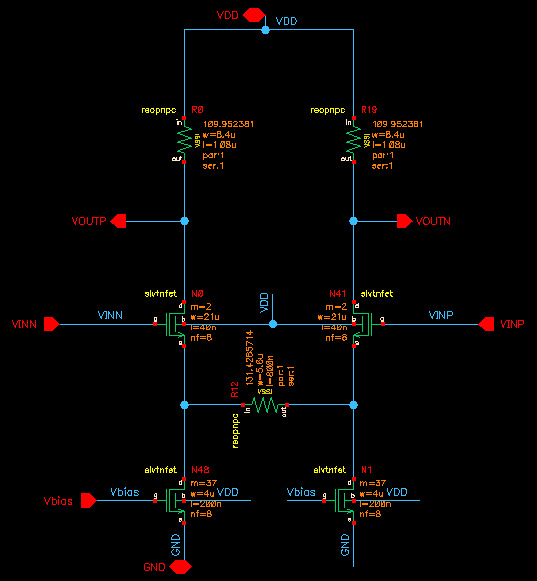
\includegraphics[width=\linewidth]{img/DFE_img/2nd GM cell.png}
        \caption{Schematic of the second $G_m$ cell.}
        \label{fig:gm_cell_2_schematic}
    \end{minipage}
\end{figure}

The DC biasing configurations for both $G_m$ cells are presented below:

\begin{figure}[H]
    \centering
    \begin{minipage}{0.48\textwidth}
        \centering
        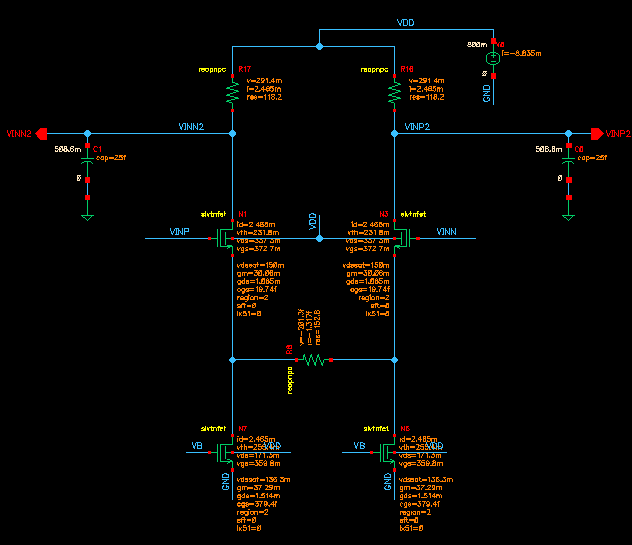
\includegraphics[width=\linewidth]{img/DFE_img/1st Gm cell biased.png}
        \caption{DC biasing of the first $G_m$ cell.}
        \label{fig:gm_cell_1_bias}
    \end{minipage}\hfill%
    \begin{minipage}{0.48\textwidth}
        \centering
        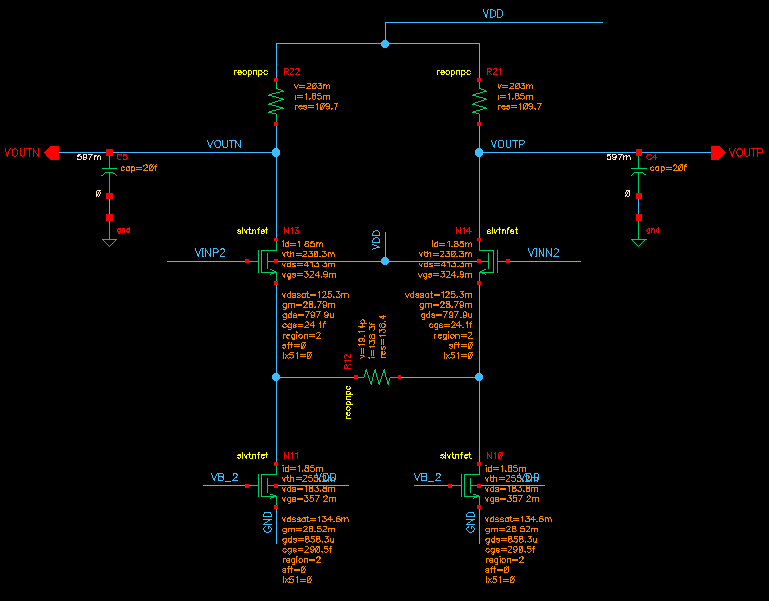
\includegraphics[width=\linewidth]{img/DFE_img/2nd Gm cell biased.png}
        \caption{DC biasing of the second $G_m$ cell.}
        \label{fig:gm_cell_2_bias}
    \end{minipage}
\end{figure}

\subsubsection{Linearity}

To evaluate the linearity of the differential pair, a DC analysis is performed where the input voltage ($V_{in}$) is swept from -300 mV to 300 mV with a step size of 20 mV. The derivative of the output voltage with respect to the input voltage is plotted to extract the voltage gain curve. The linearity region is defined and measured as the voltage range over which the gain drops by 10\% from its nominal peak value.

\begin{figure}[H]
    \centering
    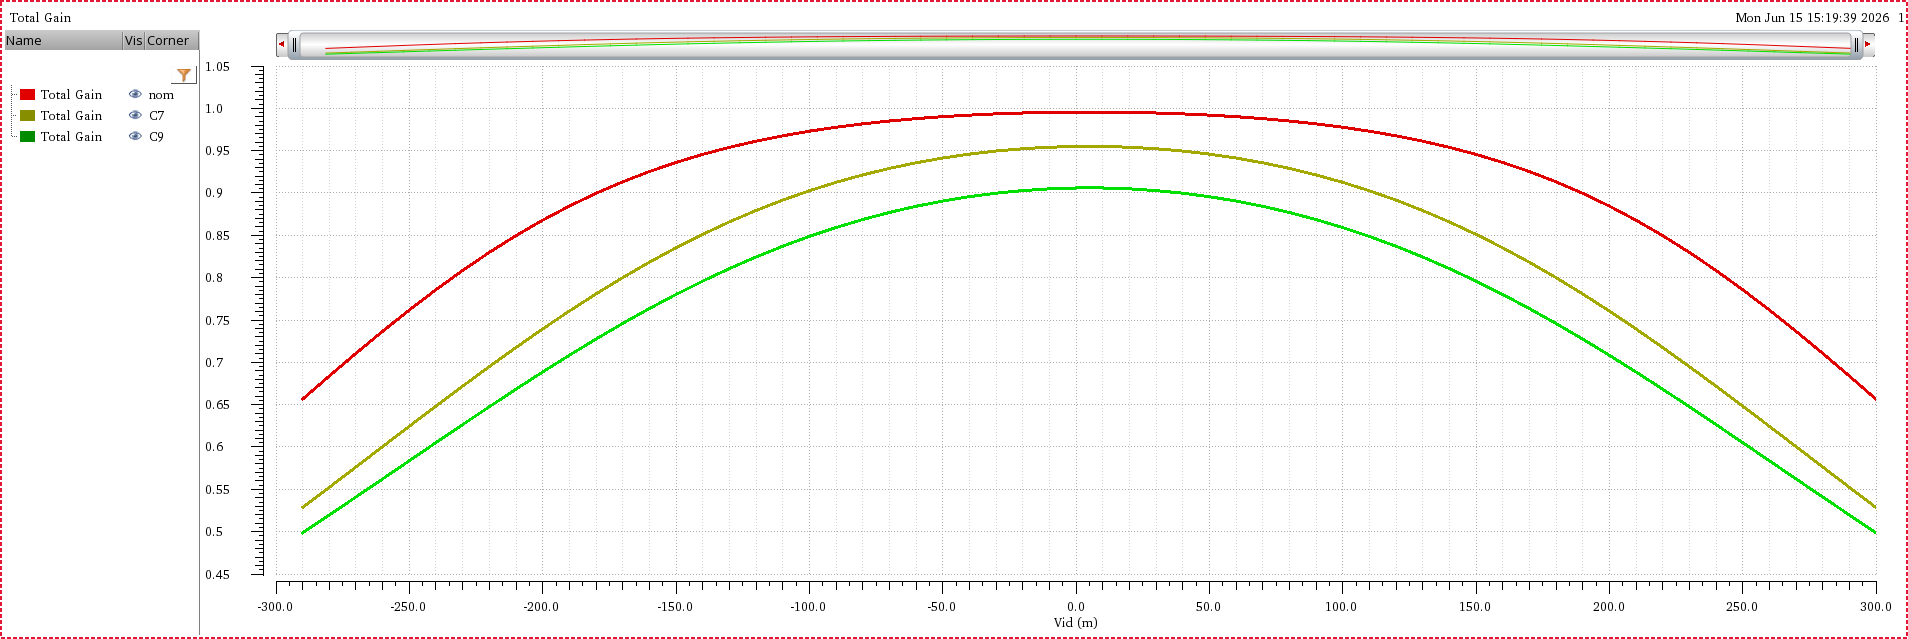
\includegraphics[width=0.8\textwidth]{img/DFE_img/Gain of 2 Gm cells.png}
    \caption{Simulated voltage gain of the differential pair across different operating corners.}
    \label{fig:diff_gain_corners}
\end{figure}

\begin{figure}[H]
    \centering
    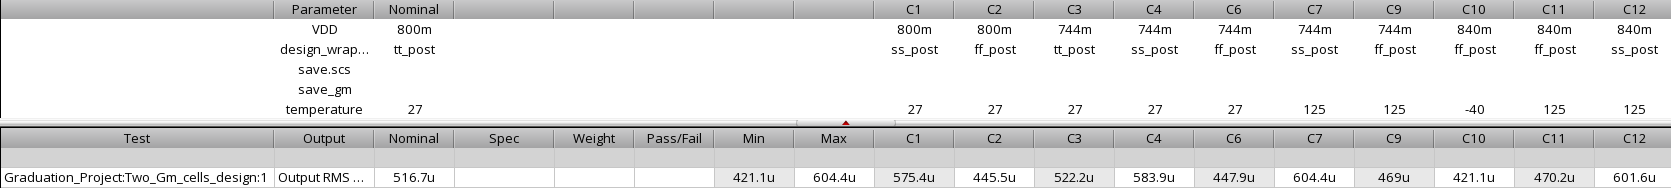
\includegraphics[width=1.2\textwidth]{img/DFE_img/output RMS noise.PNG}
    \caption{Output RMS noise voltage measured across corners.}
    \label{fig:diff_noise_corners}
\end{figure}

\begin{figure}[H]
    \centering
    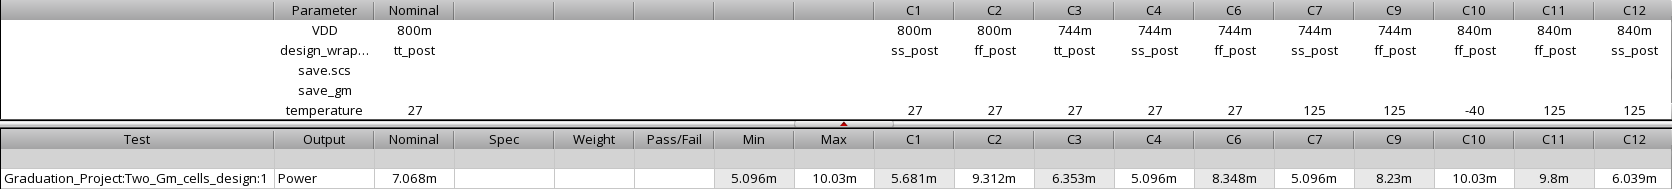
\includegraphics[width=1.2\textwidth]{img/DFE_img/Power.PNG}
    \caption{Power consumption of the differential pair across corners.}
    \label{fig:diff_power_corners}
\end{figure}

\subsection{TAP}

The testbench schematic for the DFE tap, which includes the preceding differential pair, is illustrated below. For this characterization, the first tap (T1) is set to its full-scale value. This tap is repeated 3 times because of PAM-4 signal.

\begin{figure}[H]
    \centering
    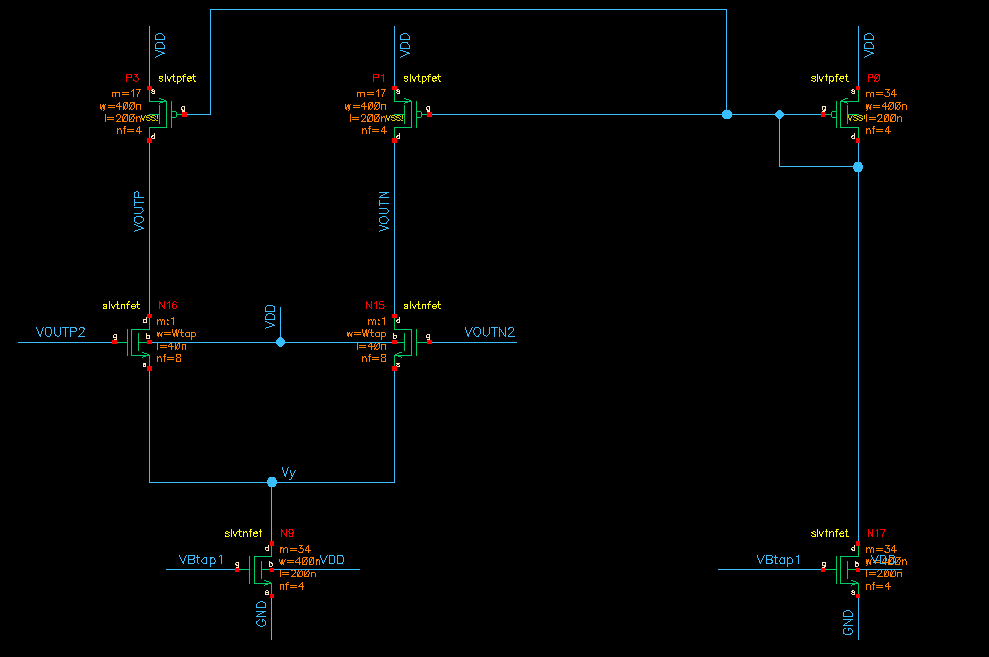
\includegraphics[width=0.9\textwidth]{img/DFE_img/Tap_sch.png}
    \caption{Testbench schematic of the tap including the differential pair.}
    \label{fig:tap_tb}
\end{figure}

A transient analysis is performed by sweeping the width of the tap transistors from 4 $\mu$m to 6 $\mu$m with a step size of 1 $\mu$m. The input signal rise and fall times ($t_r$ and $t_f$) are both set to 25 ps. 

As the transistor width increases,  ($g_m/I_D$) increases, which consequently reduces the required gate-to-source voltage ($V_{GS}$). Because of this reduced $V_{GS}$, the drain voltage of the tail current source increases proportionally with the transistor width. 

Furthermore, the tail current exhibits an alternating transient behavior. This variation is directly attributed to the parasitic capacitance present at the drain of the tail current source, which charge and discharge during switching events according to the relation $I = C \frac{dV}{dt}$.

\begin{figure}[H]
    \centering
    \begin{minipage}{0.48\textwidth}
        \centering
        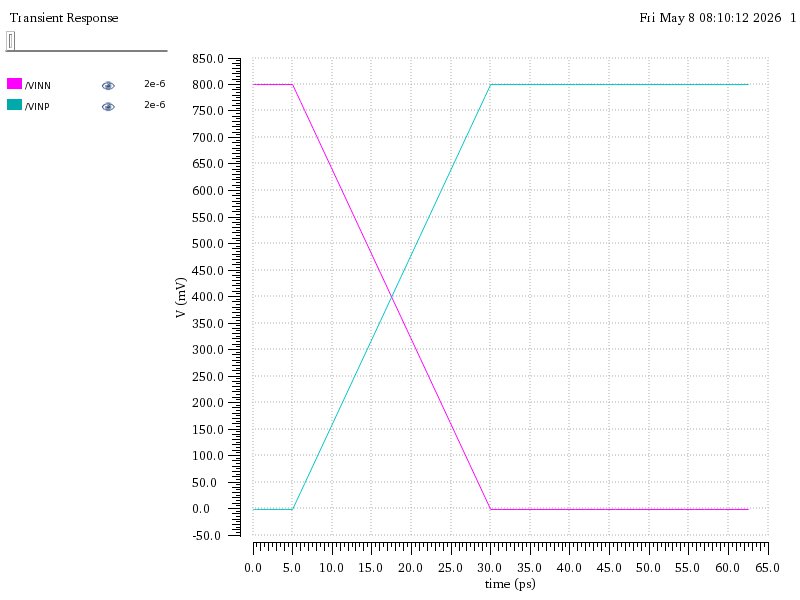
\includegraphics[width=\linewidth]{img/DFE_img/Inputs.png}
        \caption{Transient response of the input voltages ($V_{INP}$ and $V_{INN}$).}
        \label{fig:tap_vin}
    \end{minipage}\hfill%
    \begin{minipage}{0.48\textwidth}
        \centering
        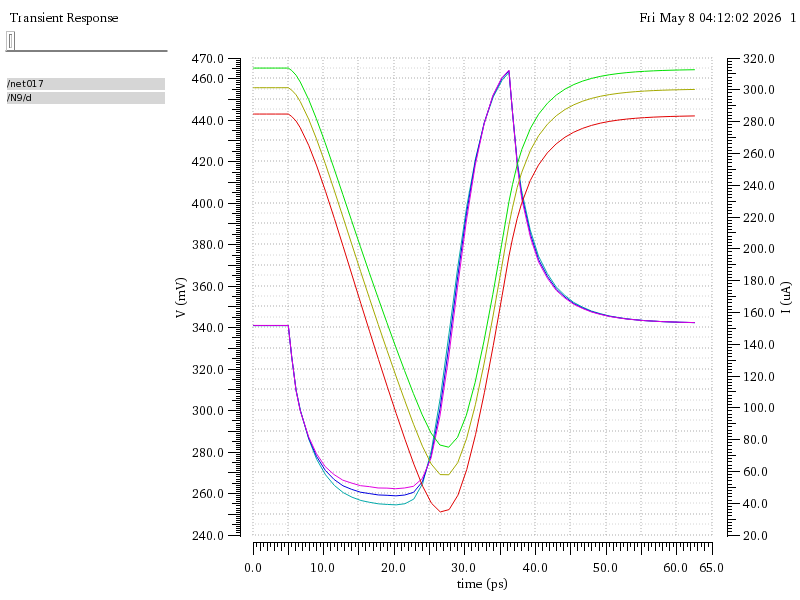
\includegraphics[width=\linewidth]{img/DFE_img/Vx & Itotal.png}
        \caption{Drain voltage of the tail current source and its corresponding current.}
        \label{fig:tap_tail}
    \end{minipage}

    \vspace{0.5cm}

    \begin{minipage}{0.6\textwidth}
        \centering
        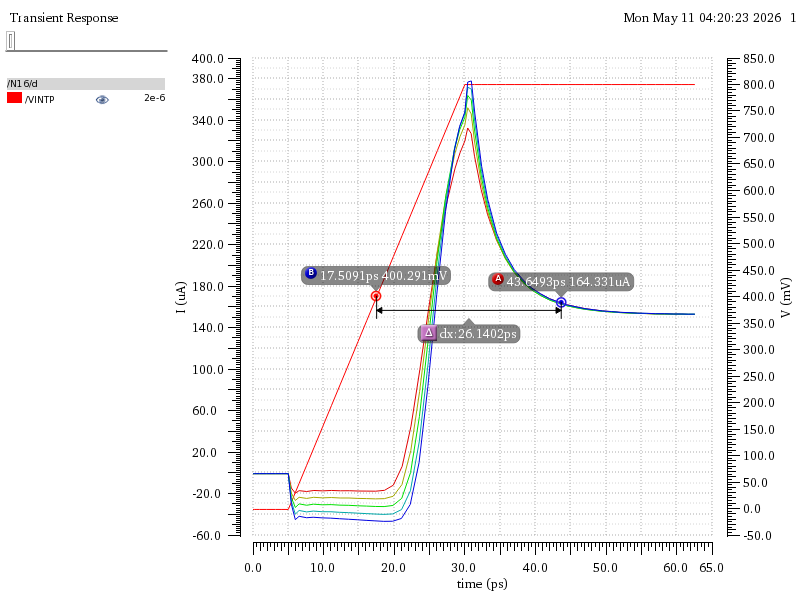
\includegraphics[width=\linewidth]{img/DFE_img/Vinp and Ip when rise time equals 25p.png}
        \caption{Transient waveforms of $V_{INP}$ and the positive tap output current ($I_p$).}
        \label{fig:tap_vinp_ip}
    \end{minipage}
\end{figure}

\subsubsection{1st Tap Simulation after Azita Comparator}

To evaluate the dynamic performance of the first tap (T1), a transient simulation is performed with the tap integrated immediately following the Azita comparator. The resulting transient waveforms demonstrate the current switching behavior, specifically highlighting the tail current and the differential output current ($I_p - I_n$).

\begin{figure}[H]
    \centering
    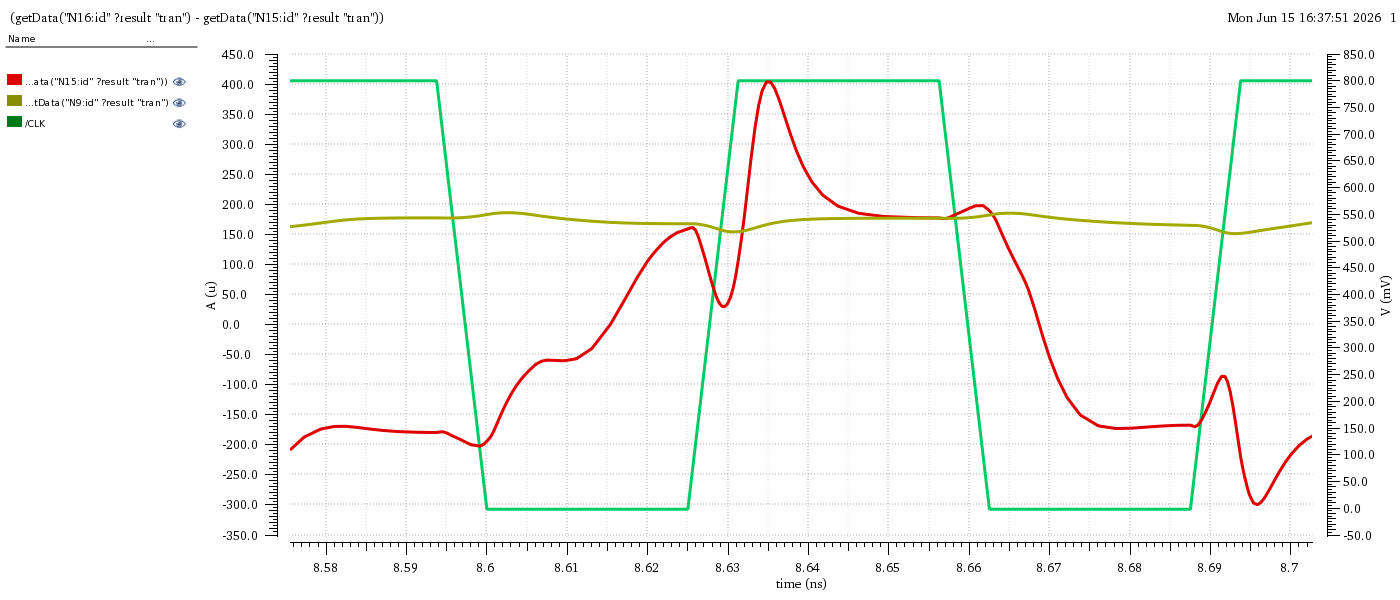
\includegraphics[width=\textwidth]{img/DFE_img/Real tap simulation.png}
    \caption{Transient simulation of the first tap cascaded after the Azita comparator (Red: Tail current, Yellow: $I_p - I_n$).}
    \label{fig:tap1_after_azita}
\end{figure}

\subsubsection{1st Tap Simulation at Worst Corner}

To guarantee the robustness of the equalization under process, voltage, and temperature variations, the first tap is also simulated at the identified worst-case corner. The transient current waveforms confirm that the tap maintains appropriate switching characteristics and drive strength even under degraded conditions.

\begin{figure}[H]
    \centering
    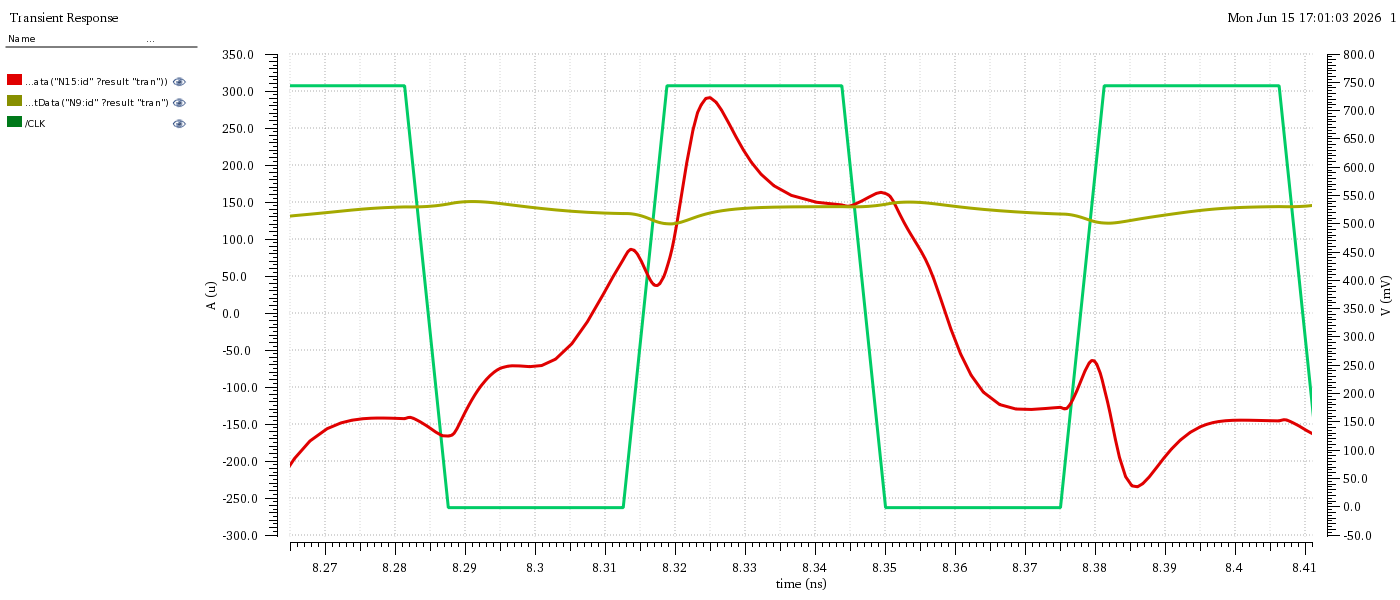
\includegraphics[width=\textwidth]{img/DFE_img/Real tap simulation_worst_corner.png}
    \caption{Transient simulation of the first tap under worst-case corner conditions (Red: Tail current, Yellow: $I_p - I_n$).}
    \label{fig:tap1_worst_corner}
\end{figure}

\subsubsection{Output Noise Across Corners}

The integrated output RMS noise of the tap structure is evaluated across the defined operating simulation corners to ensure it meets the overall signal-to-noise ratio requirements of the decision feedback equalizer.

\begin{figure}[H]
    \centering
    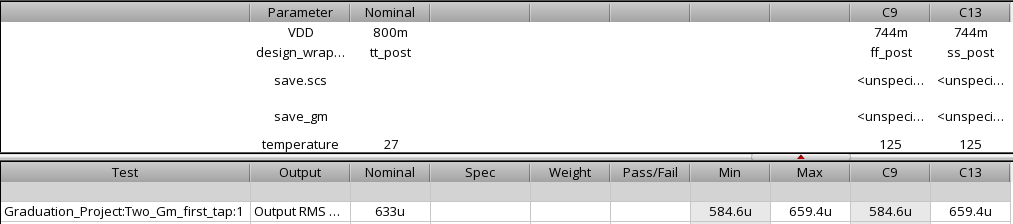
\includegraphics[width=\textwidth]{img/DFE_img/Noise across corner.PNG}
    \caption{Output RMS noise variations for the tap structure across all operating corners.}
    \label{fig:tap_noise_corners}
\end{figure}

\subsection{Thermometer-to-Binary (T2B) Decoder}

The proposed T2B decoder is implemented efficiently using multiplexer (MUX) logic. In this configuration, the intermediate thermometer code ($V_M$) is assigned directly  to the Most Significant Bit (MSB). Additionally, $V_M$ functions as the selection signal for MUX, toggling between the high ($V_H$) and low ($V_L$) thermometer states to determine and overwrite the Least Significant Bit (LSB).

\begin{figure}[H]
    \centering
    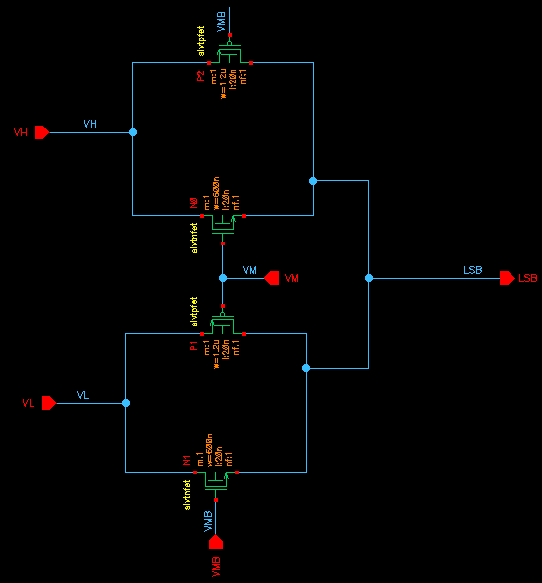
\includegraphics[width=0.6\textwidth]{img/DFE_img/T2B.png}
    \caption{Schematic of the multiplexer-based T2B decoder.}
    \label{fig:t2b_schematic}
\end{figure}

To verify the logic functionality, a transient simulation is performed where $V_H$ is forced to alternate while both $V_L$ and $V_M$ are held at a constant logic high ('1'). Under these specific input conditions, the LSB alternates successfully  in direct response to $V_H$, confirming the accurate operation of the MUX data path. 

Furthermore, this testbench is utilized to comprehensively measure the propagation delay of the T2B decoder to ensure it meets the stringent timing constraints of the DFE feedback loop.

\begin{figure}[H]
    \centering
    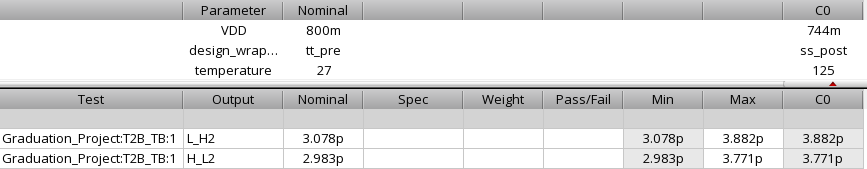
\includegraphics[width=\textwidth]{img/DFE_img/VH alternating.PNG}
    \caption{Simulation results demonstrating the measured T2B decoder propagation delay.}
    \label{fig:t2b_delay}
\end{figure}

\subsection{Calibration Loop}

As demonstrated in the methodology by [Ken Chang JSSC'17], the calibration loop is typically implemented after the deserializer (DES) in the digital domain, operating at a lower clock frequency. The data and error signals are first passed to a Pseudo-Random Binary Sequence (PRBS) checker to evaluate the Bit Error Rate (BER) and assess the quality of the adaptation. A data buffer is subsequently utilized, as the external FPGA cannot continuously receive or process every incoming word immediately. Finally, the buffered data is routed to an off-chip FPGA, which generates the binary-coded control signals necessary to adjust the DFE taps and the decision levels ($dLev$), followed by a Digital-to-Analog Converter (DAC).

\begin{figure}[H]
    \centering
    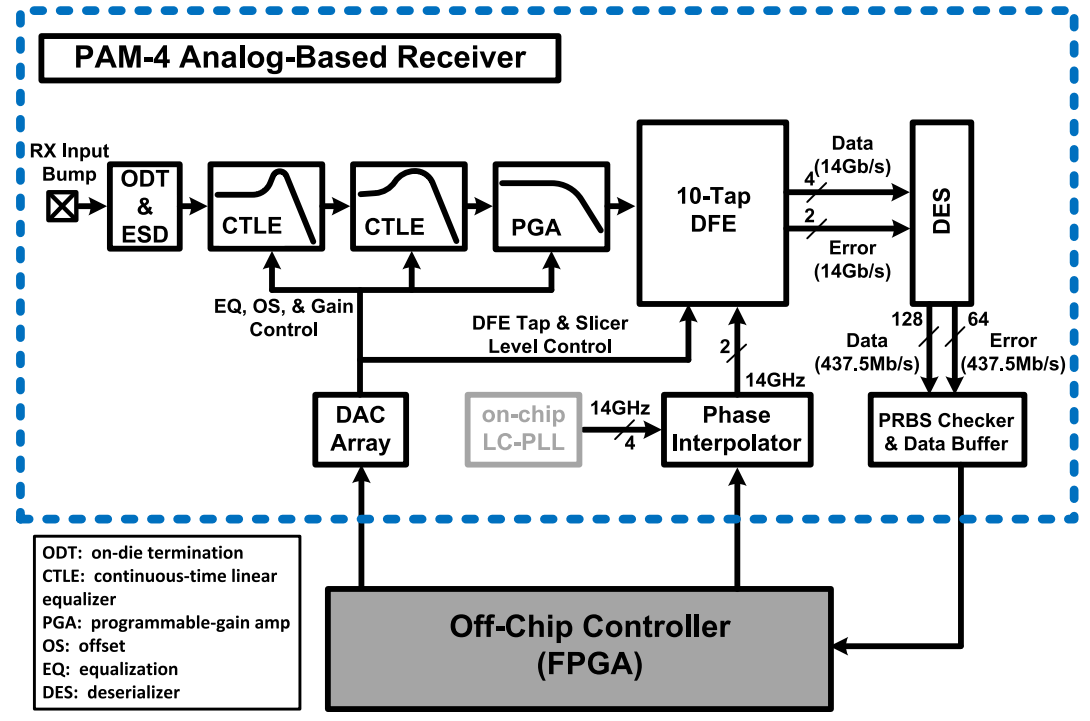
\includegraphics[width=0.6\textwidth]{img/DFE_img/Block diagram.PNG}
    \caption{Block diagram of the digital calibration and adaptation loop.}
    \label{fig:cal_loop_block}
\end{figure}

Because a DES is not implemented in this specific design phase, a simplified calibration loop specifically for the decision levels ($dLev$) is implemented directly within the high-speed analog domain. To minimize loading on the main signal path, the error signal is strategically tapped after the third latch, distancing the adaptation circuitry from the sensitive, critical timing nodes. An accumulator then processes this signal, evaluating the sign of the error to determine whether to appropriately increment or decrement the $dLev$ value.

The adaptation algorithm governing the high-level decision threshold ($dLev_H$) is defined by the following equations:
\begin{align}
    Err_H &= \text{sign}(x_{c} - dLev_H) \\
    dLev_H(n+1) &= dLev_H(n) + \mu \cdot Err_H \cdot D_H
\end{align}
\begin{figure}[H]
    \centering
    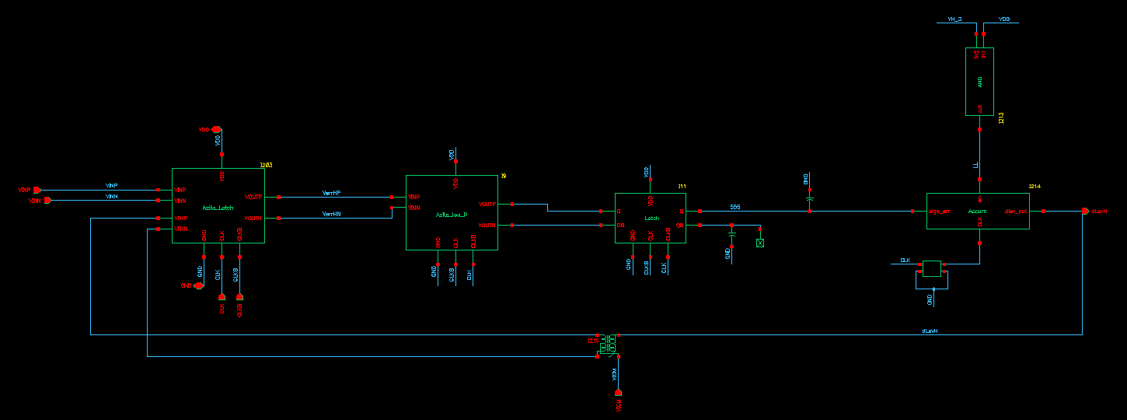
\includegraphics[width=0.9\textwidth]{img/DFE_img/Calibration_TB.png}
    \caption{Testbench schematic of the high-speed adaptation loop.}
    \label{fig:adaptation_tb}
\end{figure}

\subsubsection{High-Level Decision Threshold $dLev_H$}

The transient settling behavior of the $dLev_H$ calibration loop is illustrated below.

\begin{figure}[H]
    \centering
    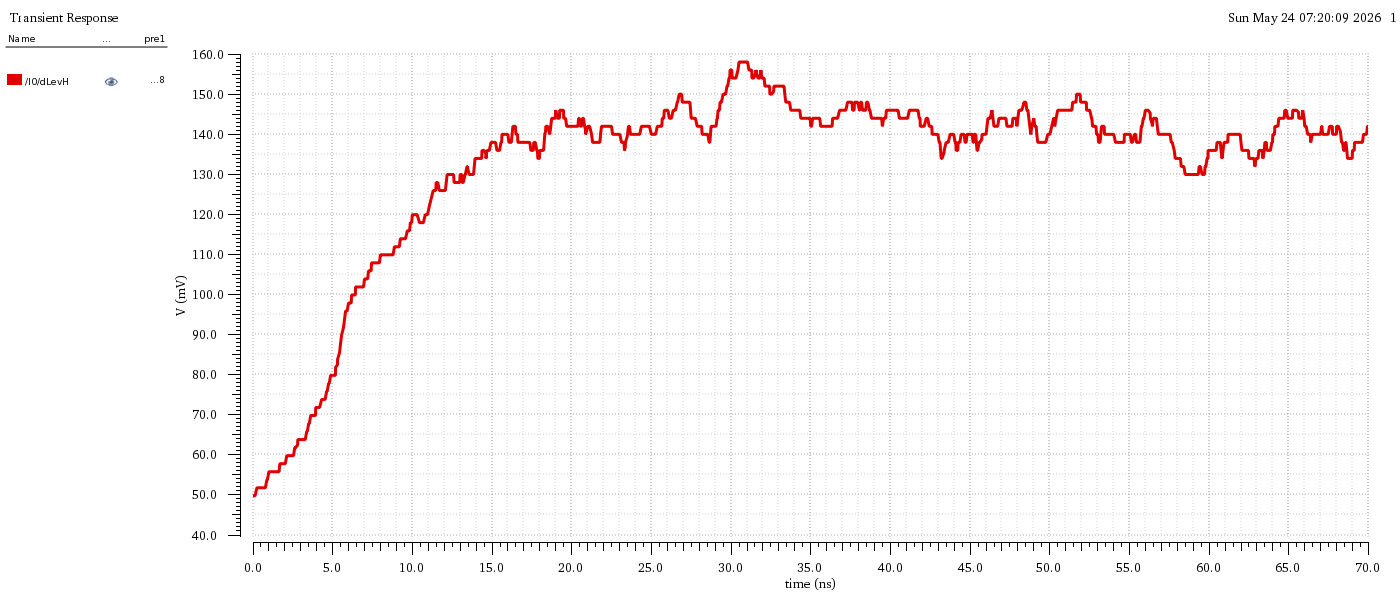
\includegraphics[width=0.8\textwidth]{img/DFE_img/LevH.png}
    \caption{Transient simulation results demonstrating the settling of the $dLev_H$ threshold.}
    \label{fig:dlevh_sim}
\end{figure}

\section{DFE Pre-Simulation Results}

\subsection{TX}

In the transmitter (TX) setup, a Pseudo-Random Binary Sequence (PRBS) voltage source is first utilized to generate a random PAM-4 test signal. Subsequently, a behavioral Feed-Forward Equalizer (FFE) block, implemented using Verilog-A, is applied to actively cancel the first pre-cursor. Due to the unavailability of the final target channel model during this phase of the design, post-cursors up to the fifth tap are manually introduced to thoroughly evaluate the DFE performance. Finally, a 50 $\Omega$ termination resistance is included to ensure proper impedance matching.

\begin{figure}[H]
    \centering
    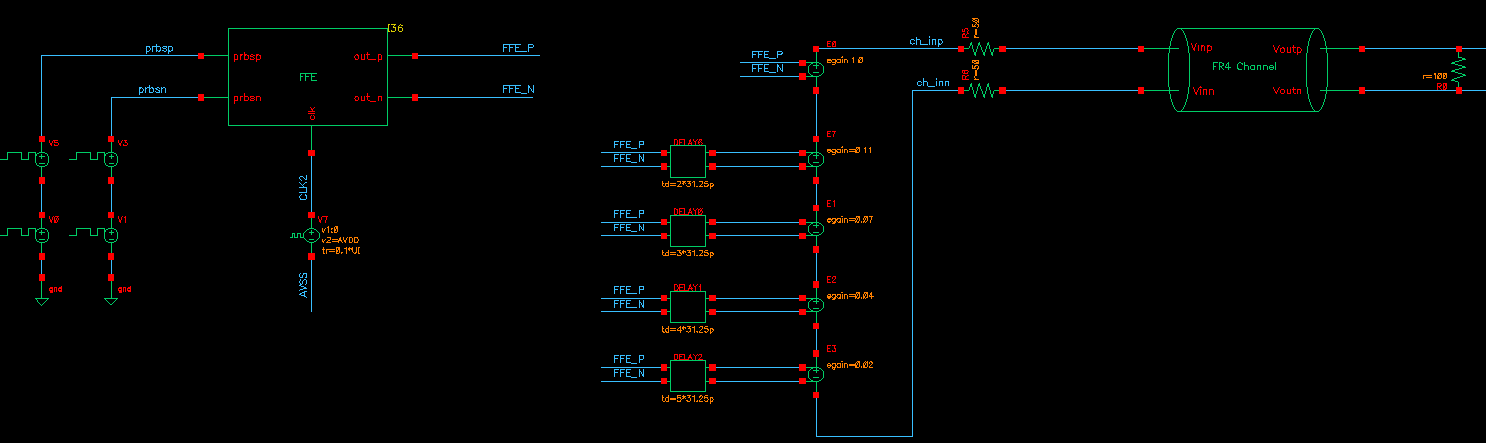
\includegraphics[width=0.8\textwidth]{img/DFE_img/TX.tb.png}
    \caption{Schematic of the TX testbench setup generating the PAM-4 signal with FFE.}
    \label{fig:tx_tb}
\end{figure}

\subsection{Channel}

The transmission channel is modeled using cascaded FR4 transmission line cells. This specific configuration is designed to exhibit a total insertion loss of 26.5 dB at the Nyquist frequency of 16 GHz.

\begin{figure}[H]
    \centering
    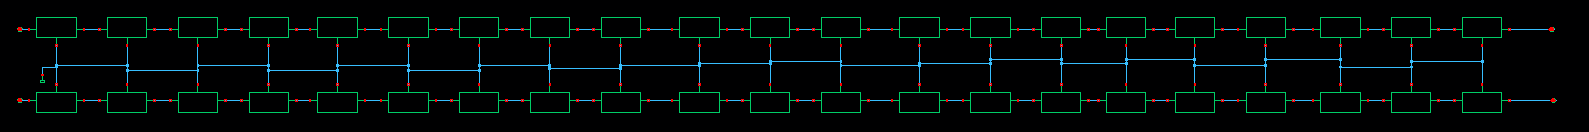
\includegraphics[width=\textwidth]{img/DFE_img/Cascaded FR4 cells.PNG}
    \caption{Schematic of the modeled FR4 channel.}
    \label{fig:channel_tb}
\end{figure}

\subsection{RX}

The receiver (RX) testbench incorporates a behavioral Continuous-Time Linear Equalizer (CTLE) at the front end. This is immediately followed by the top-level DFE block, an integrated clock buffer, and two ideal current sources utilized for biasing the equalization networks.

\begin{figure}[H]
    \centering
    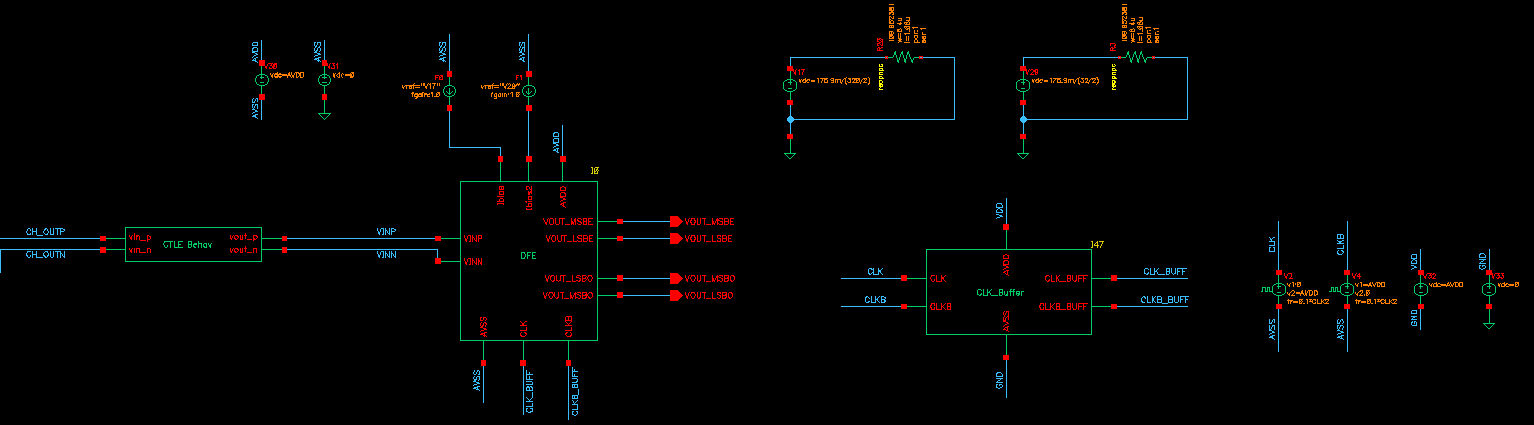
\includegraphics[width=\textwidth]{img/DFE_img/RX.tb.png}
    \caption{Schematic of the RX testbench including the behavioral CTLE and the DFE top block.}
    \label{fig:rx_tb}
\end{figure}

\subsection{DFE}

The structural configurations and specific implementation details for the DFE blocks are presented below. 

\begin{figure}[H]
    \centering
    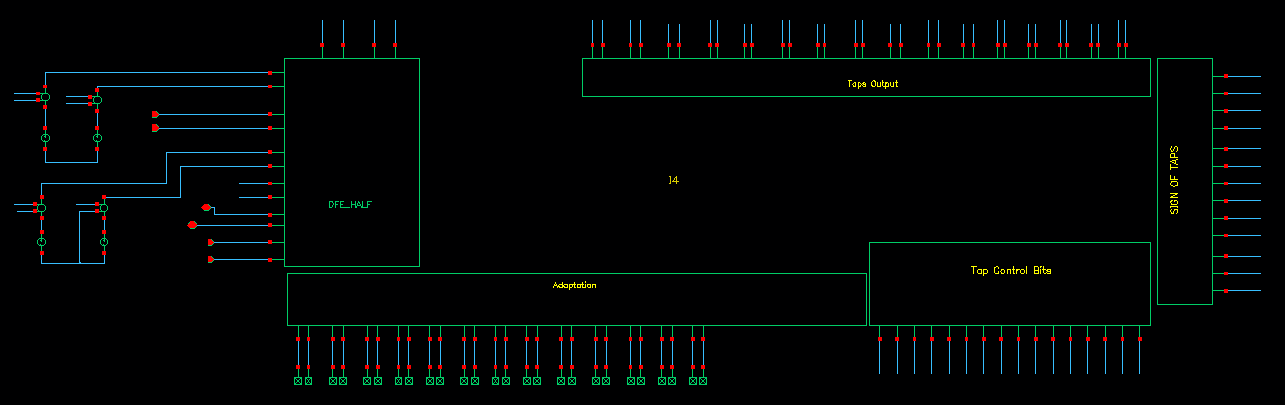
\includegraphics[width=\textwidth]{img/DFE_img/DFE even path.PNG}
    \caption{Testbench configuration of a single DFE data path.}
    \label{fig:single_path_tb}
\end{figure}

\begin{figure}[H]
    \centering
    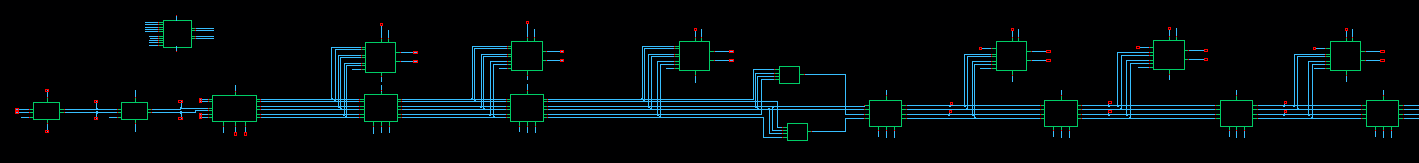
\includegraphics[width=\textwidth]{img/DFE_img/Even Path schematic.PNG}
    \caption{Detailed internal schematic of a single DFE path.}
    \label{fig:single_path_schematic}
\end{figure}

\begin{figure}[H]
    \centering
    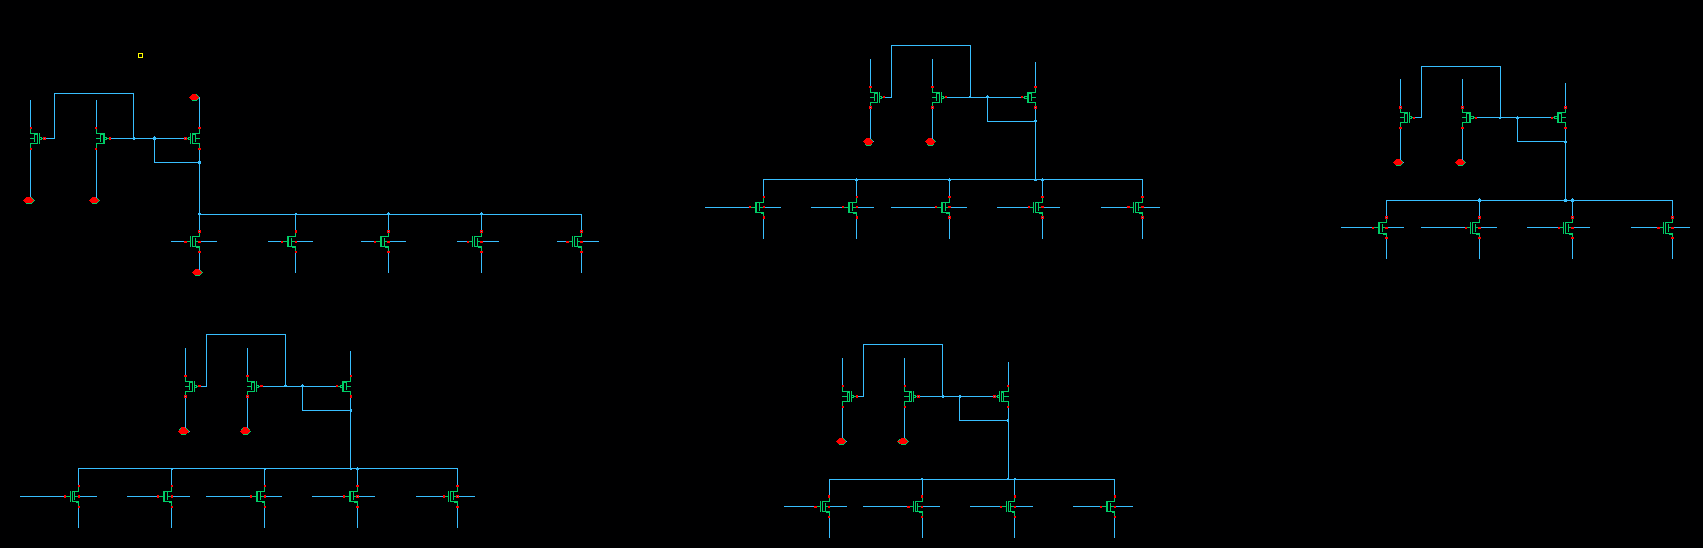
\includegraphics[width=0.8\textwidth]{img/DFE_img/Compensation Loop.PNG}
    \caption{Schematic detailing the common mode compensation network.}
    \label{fig:cm_compensation}
\end{figure}

\subsubsection{Performance with 2-Tap Post-Cursor Cancellation}

Initial performance is evaluated over a channel with an insertion loss of 26.5 dB, configuring the DFE to cancel only the first two post-cursors. The resulting eye diagrams observed after the CTLE and at the summing node are presented below.
Eye height = 66 mV
\begin{figure}[H]
    \centering
   
        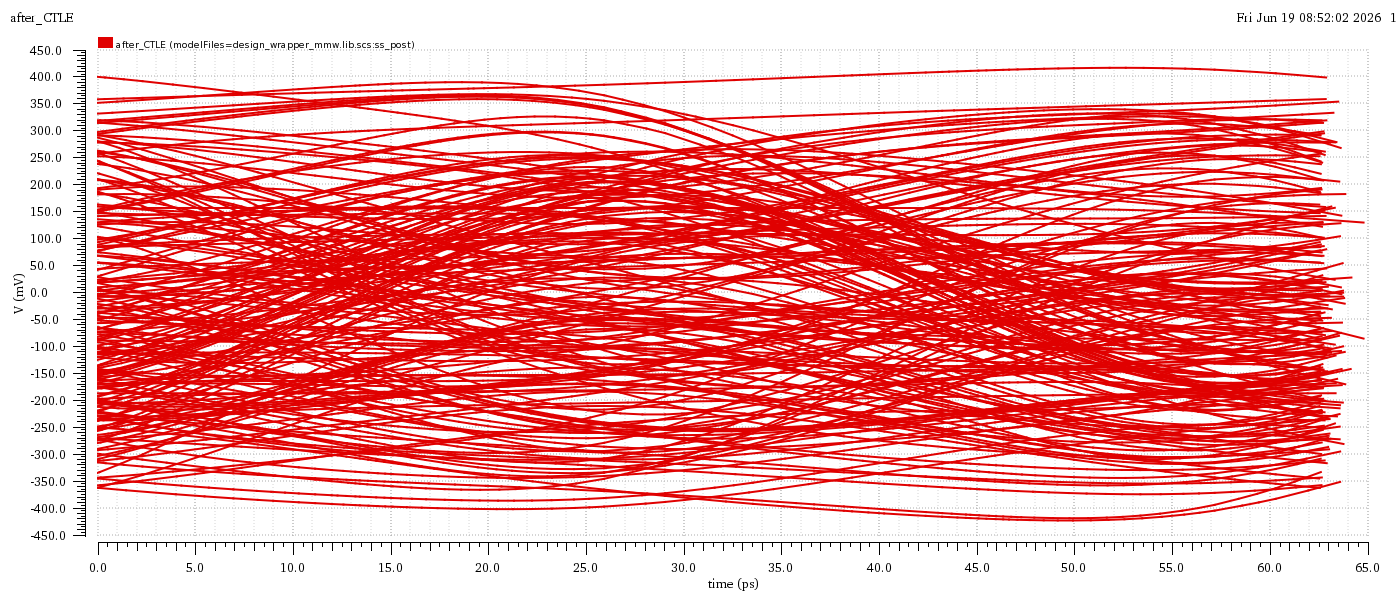
\includegraphics[width=\linewidth]{img/DFE_img/After CTLE_2.png}
        \caption{Eye diagram after the CTLE (2 post-cursors cancelled).}
        \label{fig:eye_ctle_2taps}
\end{figure}
    \begin{figure}[H]
        \centering
        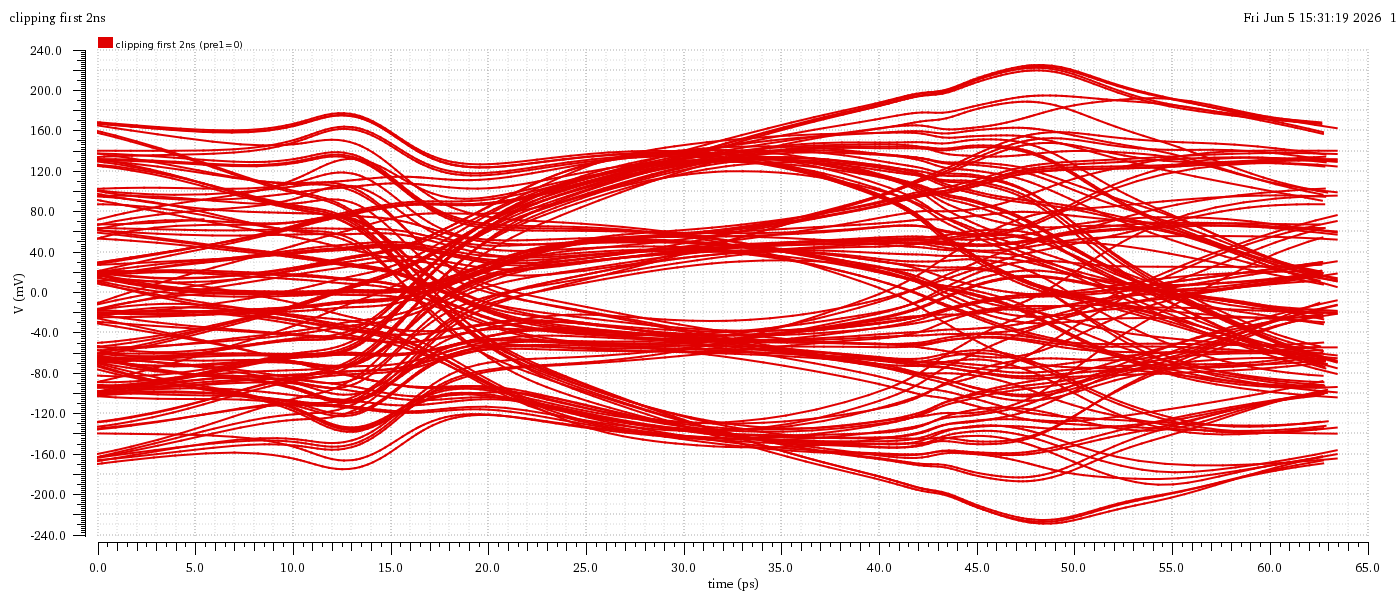
\includegraphics[width=\linewidth]{img/DFE_img/only 2 post cursors taps.png}
        \caption{Eye diagram at the summing node (2 post-cursors cancelled).}
        \label{fig:eye_summer_2taps}
\end{figure}

\subsubsection{Performance with 5-Tap Post-Cursor Cancellation}

To further optimize the equalization for the 26.5 dB channel, five post-cursors are manually introduced. In this configuration, the equalization effectively cancels the first pre-cursor alongside the first five post-cursors. The Single Bit Response (SBR) at the summer node is extracted to verify the cancellation limits.
Eye height = 60.8 mV
\begin{figure}[H]
    \centering
    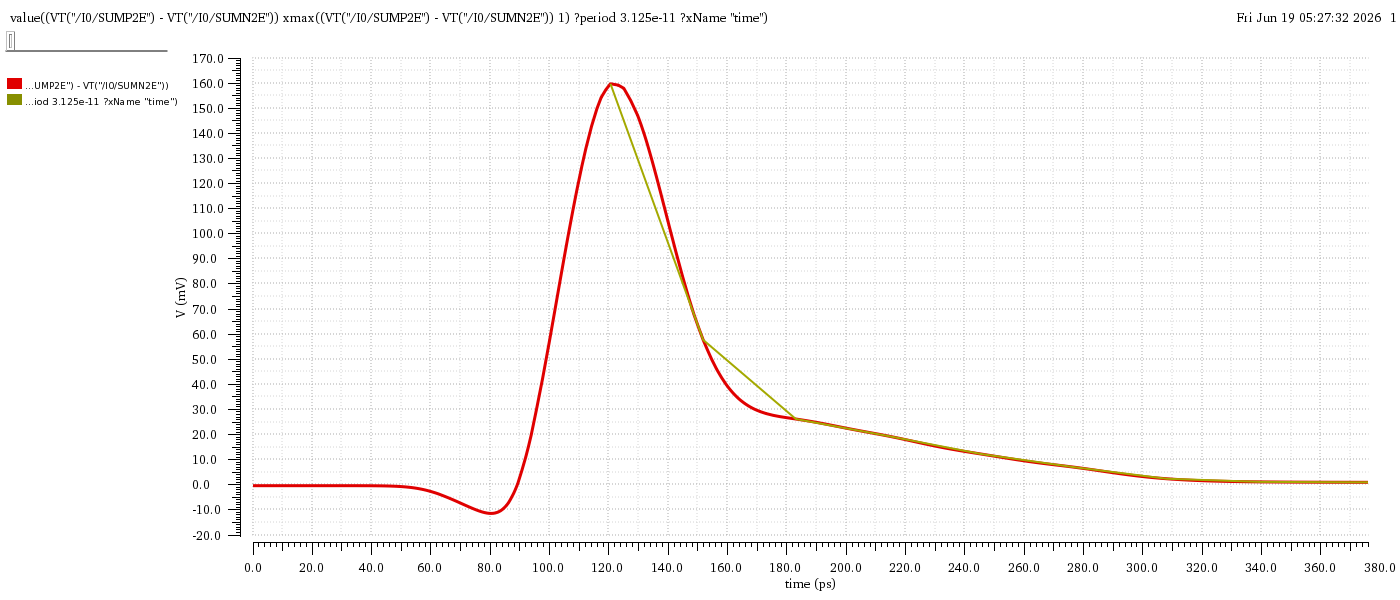
\includegraphics[width=0.8\textwidth]{img/DFE_img/SBR.png}
    \caption{Single Bit Response (SBR) at the summer node after manual cursor addition.}
    \label{fig:sbr_5taps}
\end{figure}

The corresponding eye diagrams demonstrate the improved signal integrity and widened eye opening achieved through this expanded tap configuration.

\begin{figure}[H]
    \centering
        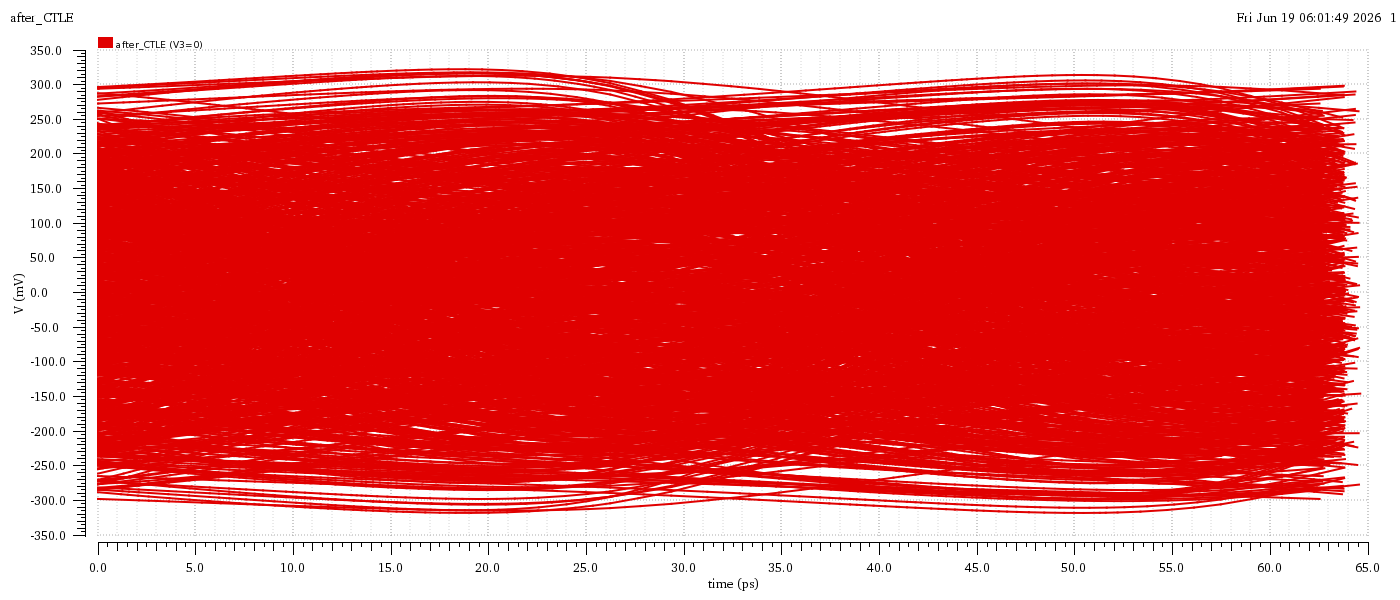
\includegraphics[width=\linewidth]{img/DFE_img/after CTLE.png}
        \caption{Eye diagram after the CTLE (5 post-cursors cancelled).}
        \label{fig:eye_ctle_5taps}
        \end{figure}
        \begin{figure}[H]
    \
        \centering
        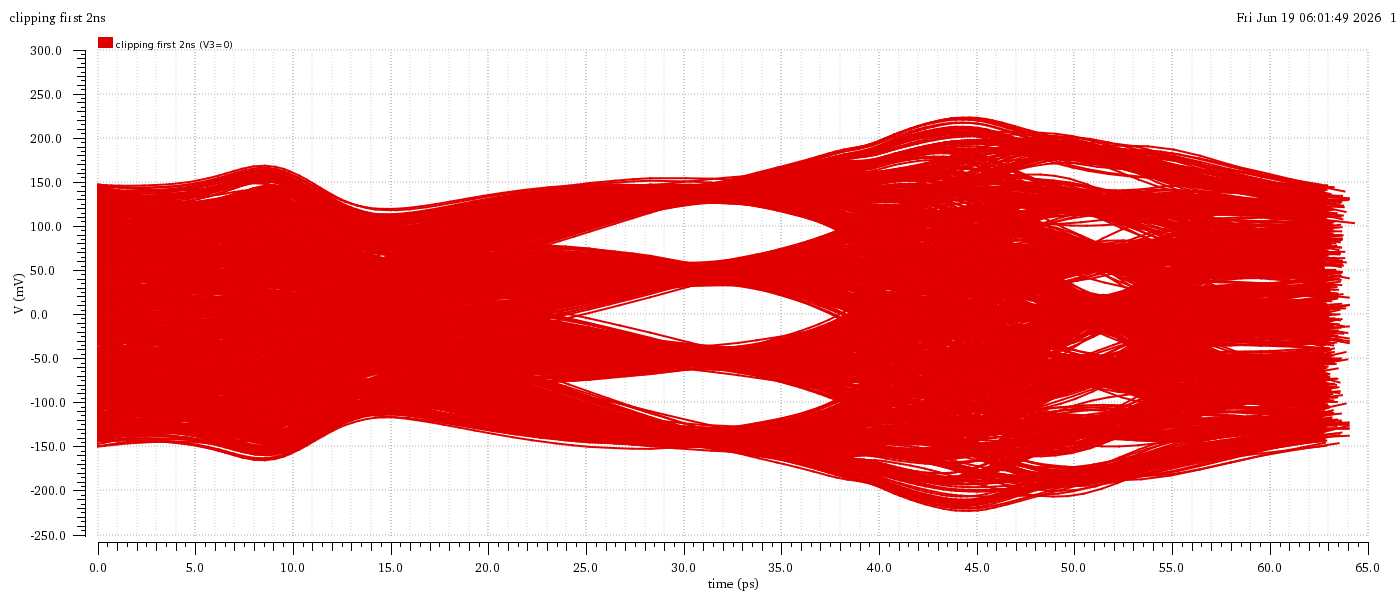
\includegraphics[width=\linewidth]{img/DFE_img/DFE results of 5 taps and pre-cursor.png}
        \caption{Eye diagram at the summing node (5 post-cursors cancelled).}
        \label{fig:eye_summer_5taps}
\end{figure}

4 levels can be detected from the eye diagram of the output of the middle comparator
\begin{figure}[H]
    \
        \centering
        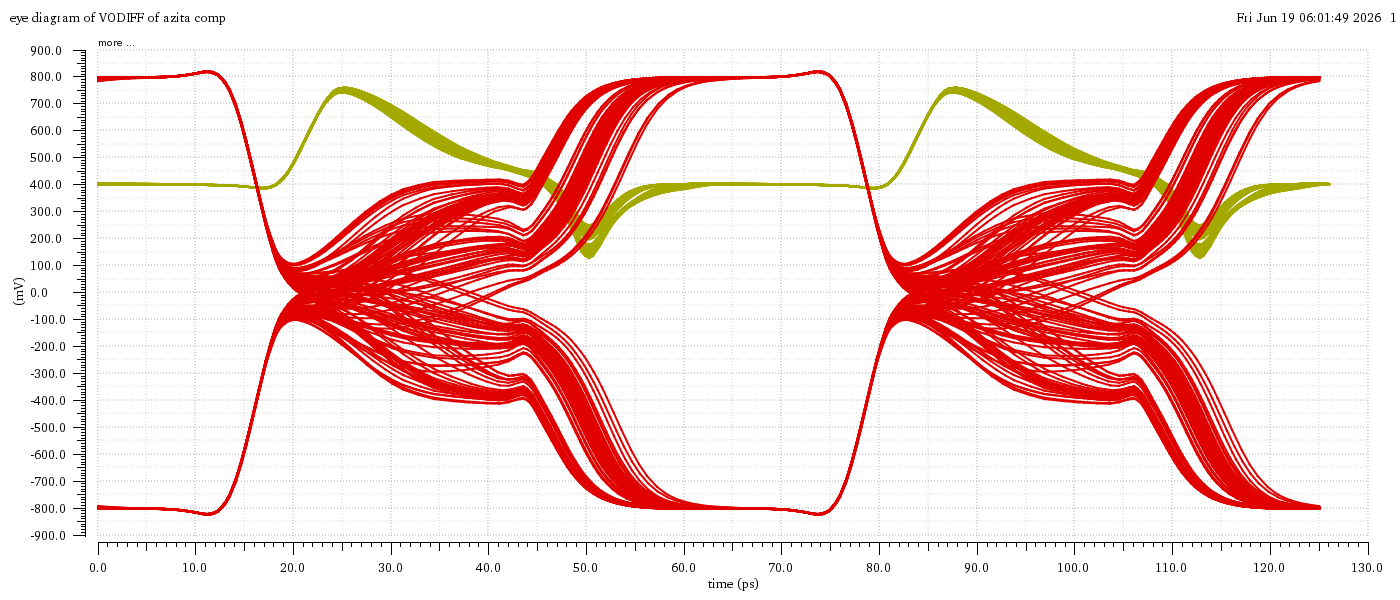
\includegraphics[width=\linewidth]{img/DFE_img/Eye diagram of VODIFF and VOCM of middle comparator.png}
        \caption{Eye diagram of output of middle comparator}
        \label{Eye diagram of output of middle comparator}
\end{figure}

\subsubsection{Noise Contributors}

The overall noise performance of the system is determined by the individual contributions from each major sub-block. Table \ref{tab:noise_contributors} summarizes the integrated noise contributed by the analog front end, the slicers, and the $G_m$ cells, which combine to yield a total system noise of 2.88 mV.

\begin{table}[H]
    \centering
    \caption{Summary of noise contributors across different structural blocks.}
    \label{tab:noise_contributors}
    \renewcommand{\arraystretch}{1.2} % Adds a little padding to the rows for readability
    \begin{tabular}{|c|c|c|c|c|}
        \hline
        \textbf{Block} & \textbf{Analog front end} & \textbf{Slicers} & \textbf{2 Gm cells} & \textbf{Total} \\
        \hline
        Noise & 1.514 mV & 2.4 mV & 0.517 mV & 2.88 mV \\
        \hline
    \end{tabular}
\end{table}

\begin{figure}[H]
    \centering
    \includegraphics[width=\textwidth]{img/DFE_img/bathtub.png}
    \caption{Bathtub diagram for the Typical case.}
    \label{fig:bathtub_typical}
\end{figure}


\subsubsection{Worst-Case Corner Performance}

Finally, the robustness of the equalization scheme is verified under the worst-case operating corner. This stringent corner is defined by the slow-slow (SS) process variation, an elevated temperature of $125^\circ\text{C}$, and a degraded supply voltage ($V_{DD}$) of 0.752 V, which represents 94\% of the nominal supply.

\begin{figure}[H]
    \centering
    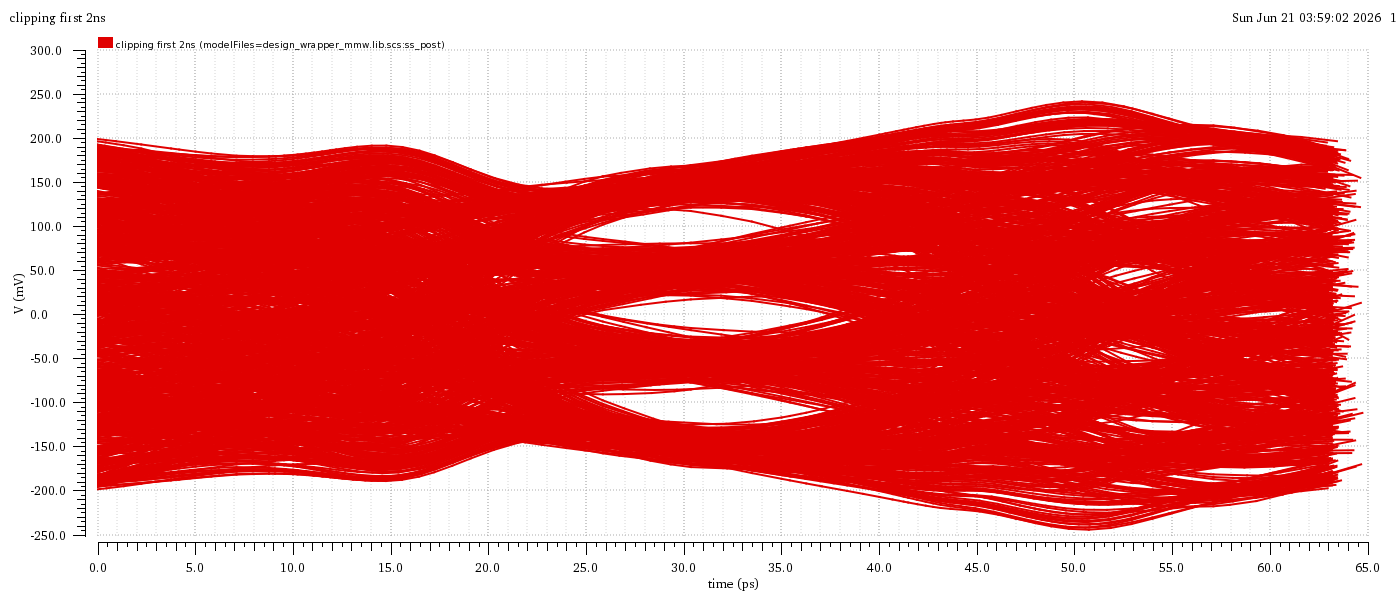
\includegraphics[width=\textwidth]{img/DFE_img/eye diagram for worst cursors.png}
    \caption{Eye diagram at the summing node under worst-case corner conditions (SS, $125^\circ\text{C}$, 0.752 V).}
    \label{fig:eye_summer_worst_corner}
\end{figure}
